\documentclass[11pt,a4paper]{article}
% \documentclass[11pt]{amsart}
\usepackage[utf8]{inputenc}
\usepackage[margin=1in]{geometry}
\usepackage{color}
\usepackage{graphicx}
\usepackage{microtype}
\usepackage{array}
\usepackage{verbatim}
\usepackage{caption}
\usepackage{subcaption}
\usepackage{amsmath,amsthm,amsfonts,amssymb,latexsym}
\usepackage{bbm}
\usepackage{setspace}
\usepackage{xparse}
\usepackage{epstopdf}
\usepackage{pgf}
\usepackage[colorlinks=true,citecolor=blue]{hyperref}
\usepackage[nameinlink,capitalise]{cleveref}

\usepackage[style=trad-abbrv,doi=false,url=false,isbn=false,backend=biber]{biblatex}
\DeclareFieldFormat{volume}{volume \textbf{#1}}
\DeclareFieldFormat[article]{volume}{\textbf{#1}}
\addbibresource{main.bib}

\usepackage{tikz}
\usepackage{tikz-cd}
\usepackage{pgfplotstable}
\pgfplotsset{compat=1.14}
\usetikzlibrary{patterns}
\usetikzlibrary{calc}
\usetikzlibrary{angles}
\usetikzlibrary{quotes}
\usetikzlibrary{external}

\onehalfspacing
% \setlength{\parskip}{6pt}

\DeclareDocumentCommand\abs{s m} {\IfBooleanTF{#1}{\left|#2\right|}{\left|#2\right|}}
\DeclareDocumentCommand\cont{o m o} {C\IfNoValueF{#1}{^{#1}}(#2\IfNoValueF{#3}{;#3})}
\DeclareDocumentCommand\contc{o m o} {C_c\IfNoValueF{#1}{^{#1}}(#2\IfNoValueF{#3}{;#3})}
\DeclareDocumentCommand\sobolev{m m o} {H^{#1}(#2 \IfNoValueF{#3}{,#3})}
\DeclareDocumentCommand\lp{m m o} {L^{#1}\left(#2 \IfNoValueF{#3}{,#3}\right)}
\DeclareDocumentCommand\norm{s m o} {\IfBooleanTF{#1}{\|#2\|}{\left\|#2\right\|}\IfNoValueF{#3}{_{#3}}}
\DeclareDocumentCommand\seminorm{m o o} {\left|#1\right|\IfNoValueF{#2}{_{#2 \IfNoValueF{#3}{,#3}}}}
\DeclareDocumentCommand\ip{s m m o} {\IfBooleanTF{#1}{\langle #2,#3 \rangle}{\left\langle #2,#3 \right\rangle}\IfNoValueF{#4}{_{#4}}}
\DeclareDocumentCommand\dup{m m o} {\left\langle{#1,#2}\right\rangle\IfNoValueF{#3}{_{#3', #3}}}
\DeclareDocumentCommand\gaussian{O{0} O{I}} {g_{#1, #2}}
\DeclareDocumentCommand\littleo{s o m} {o\IfNoValueF{#2}{_{#2}}\IfBooleanTF{#1}{(#3)}{\left(#3\right)}}
\DeclareDocumentCommand\bigo{s o m} {\mathcal O\IfNoValueF{#2}{_{#2}}\IfBooleanTF{#1}{(#3)}{\left(#3\right)}}


\DeclareMathOperator*{\argmax}{arg\,max}
\DeclareMathOperator*{\argmin}{arg\,min}
\DeclareMathOperator*{\re}{Re}
\DeclareMathOperator*{\trace}{tr}
\DeclareMathOperator{\Span}{span}
\DeclareMathOperator{\sym}{sym}
\DeclareMathOperator{\sign}{sign}
\DeclareMathOperator{\diag}{diag}
\DeclareMathOperator{\id}{id}

% \DeclareMathOperator{\e}{e}
\newcommand{\e}{\mathrm{e}}

\newcommand{\revision}[1]{\textcolor{blue}{#1}}
\renewcommand{\revision}[1]{#1}
\newcommand{\gab}[1]{\textcolor{darkgreen}{#1}}
\newcommand{\commut}[2]{[#1, #2]}
\newcommand{\laplacian}{\Delta}
\newcommand{\correlation}[1]{\left< #1 \right>}
\newcommand{\dummy}{\,\cdot\,}
\newcommand{\expect}[0]{\mathbf{E}}
\newcommand{\proba}[0]{\mathbf{P}}
\newcommand{\var}[0]{\mathbf{V}}
\newcommand{\iip}[2]{\left(\!\left(#1, #2\right)\!\right)}
\newcommand{\nat}{\mathbf N}
\newcommand{\poly}{\mathbf P}
\newcommand{\real}{\mathbf R}
\newcommand{\integer}{\mathbf Z}
\newcommand{\torus}{\mathbf T}
\newcommand{\grad}{\nabla}
\newcommand{\imag}{\mathrm{i}}
\newcommand{\hess}{\nabla^2}
\newcommand{\vect}[1]{\boldsymbol{\mathbf #1}}
\newcommand{\mat}[1]{\vect #1}
\renewcommand{\det}[1]{\mathrm{det} \left( #1 \right)}
\renewcommand{\d}{\mathrm d}
\renewcommand{\t}{\mathsf T}
% \renewcommand{\t}{t}

\makeatletter
\DeclareDocumentCommand \derivative{s m o m}{%
    \def\@der{\IfBooleanTF{#1}{\mathrm{d}}{\partial}}
    \def\@default{%
        \mathchoice{%
                \frac{%
                    \@der\ifnum\pdfstrcmp{#2}{1}=0\else^{#2}\fi {\IfNoValueTF{#3}{}{#3}}
                }{%
                    \@for\@token:={#4}\do{\@der \@token}
                }
            } {%
                \@for\@token:={#4}\do{\@der_\@token} \IfNoValueTF{#3}{}{#3}
            } {} {}
    }
    \IfBooleanTF{#1}{\IfNoValueTF{#3}{\@default}{%
                #3%
                \ifnum\pdfstrcmp{#2}{1}=0'\else%
                \ifnum\pdfstrcmp{#2}{2}=0''\else%
                \ifnum\pdfstrcmp{#2}{3}=0^{(3)}\else%
                \ifnum\pdfstrcmp{#2}{4}=0^{(4)}\else%
                \ifnum\pdfstrcmp{#2}{5}=0^{(5)}\else%
                ^{(#2)}\fi\fi\fi\fi\fi
            }
        }{\@default}
}
\makeatother

\definecolor{darkred}{rgb}{.5,0,0}
\definecolor{darkgreen}{rgb}{0,.5,0}
\definecolor{darkblue}{rgb}{0,0,.5}
\newcommand{\red}[1]{\textcolor{darkred}{#1}}
\newcommand{\green}[1]{\textcolor{darkgreen}{#1}}

\theoremstyle{plain}
\newtheorem{assumption}{Assumption}[section]
\newtheorem{lemma}{Lemma}[section]
\newtheorem{corollary}{Corollary}[section]
\newtheorem{theorem}{Theorem}[section]
\newtheorem{proposition}{Proposition}[section]
\newtheorem{result}{Result}[section]
\newtheorem{remark}{Remark}[section]
\newtheorem{example}{Example}[section]
\numberwithin{equation}{section}

\newcounter{urbainCounter}
\newcommand{\urbain}[1]{\stepcounter{urbainCounter}\red{\arabic{urbainCounter}.} \green{#1}}
\crefname{equation}{}{}
\crefname{paragraph}{\S\!}{\S}
% \crefname{figure}{Figure}{Figures}
% \crefname{section}{Section}{Sections}

\newcommand{\email}[1]{\href{#1}{#1}}
\newcommand{\orcidcolor}{ORC\textcolor{orcidlogocol}{ID}}
\newcommand{\orcid}[1]{\href{https://orcid.org/#1}{
\includegraphics[width=.4cm]{z_orcid.pdf}}}

%---------------- GABRIEL ------------
\usepackage{enumerate}
\newcommand{\eps}{\varepsilon}
\newcommand{\dps}{\displaystyle}
\newcommand{\cX}{\mathcal{X}}
\newcommand{\ri}{\mathrm{i}}
\renewcommand{\leq}{\leqslant}
\renewcommand{\geq}{\geqslant}
\renewcommand{\le}{\leqslant}
\renewcommand{\ge}{\geqslant}
% \usepackage{todonotes}
\usepackage{mathrsfs}

% BODY {{{1
\date{\today}
\title{Mobility estimation for Langevin dynamics using control variates}
\author{%
  % G.A. Pavliotis\thanks{Department of Mathematics, Imperial College London (\email{g.pavliotis@imperial.ac.uk})}%
  % \hspace{2mm}\orcid{0000-0002-3468-9227}%
  % \and G. Stoltz\thanks{CERMICS, \'Ecole des Ponts, France \& MATHERIALS, Inria Paris (\email{gabriel.stoltz@enpc.fr})}
  % \hspace{2mm}\orcid{0000-0002-2797-5938}%
  % \and U. Vaes\thanks{Department of Mathematics, Imperial College London (until October 2020) and MATHERIALS, Inria Paris (since November 2020) (\email{urbain.vaes@inria.fr})}%
  % \hspace{2mm}\orcid{0000-0002-7629-7184}%
}

\begin{document}
\maketitle

\begin{abstract}
    The scaling of the mobility of two-dimensional Langevin dynamics in a periodic potential as the friction vanishes is not well understood for non-separable potentials.
    Theoretical results are lacking,
    and numerical calculation of the mobility in the underdamped regime is challenging because
    the computational cost of standard Monte Carlo methods is inversely proportional to the friction coefficient.
    In this note, we propose a new variance-reduction method based on control variates for efficiently estimating the mobility of Langevin-type dynamics.
    We provide bounds on the bias and variance of the proposed estimator,
    and illustrate its efficacy through numerical experiments,
    first in simple one-dimensional settings
    and then for two-dimensional Langevin dynamics.
    Our results corroborate previous numerical evidence that
    the mobility scales as~$\gamma^{-\alpha}$ in the low friction regime for a simple non-separable potential.
\end{abstract}

\section{Introduction}%
Langevin dynamics model the evolution of a system of particles interacting with an environment at fixed temperature.
They are widely used for the calculation of macroscopic properties of matter in molecular simulation.
Assuming a diagonal mass matrix,
the standard Langevin dynamics, sometimes called underdamped Langevin dynamics,
reads after appropriate non-dimensionalization~\cite[Section 2.2.4]{MR2681239}
\begin{subequations}
\label{eq:langevin}
\begin{align}
    \label{eq:langevin_q}
    \d \vect q_t &= \vect p_t \, \d t, \\
    \label{eq:langevin_p}
    \d \vect p_t &= - \grad V(q_t) \, \d t - \gamma \, \vect p_t \, \d t + \sqrt{2 \gamma \beta^{-1}} \, \d \vect w_t.
\end{align}
\end{subequations}
Here $\vect q_t \in \torus^d$ and $\vect p_t \in \real^d$ are the position and velocity variables,
with~$\torus^d = \real^d / 2\pi \integer^d$ the $d$-dimensional torus with period $2 \pi$.
Throughout this note, we emphasize vectorial quantities in bold.
The parameter $\gamma$ is a dimensionless parameter we call the friction,
$V$ is a periodic potential
and~$\vect w_t$ is a standard $d$-dimensional Brownian motion.
% $M$ is the mass matrix,
% For simplicity we assume that $M = m I_d$,
% where $I_d \in \real^{d \times d}$ is the identity matrix.
% In this case $(\widetilde q_t, \widetilde p_t) := (q_{\sqrt{m} t}, m^{-1/2} p_{\sqrt{m} t})$
% is a weak solution of~\eqref{eq:langevin} with $m = 1$ and $\gamma$ replaced by $\gamma/\sqrt{m}$,
% so to further simplify we assume $m = 1$,
% keeping in mind that asymptotic results for the case $m \neq 1$ can be deduced from this transformation;
% see~\cite[Section 2.2.4]{MR2681239} for a more detailed motivation of this simplification.
% keeping in mind that results obtained in the limit;
We recall that the dynamics~\eqref{eq:langevin} is ergodic with respect to the Boltzmann--Gibbs measure
\begin{equation}
    \label{eq:invariant_measure}
    \mu(\d \vect q \, \d \vect p) = \frac{1}{Z} \exp \bigl( - \beta H(\vect q, \vect p)  \bigr) \, \d \vect q \, \d \vect p,
    \qquad H(\vect q, \vect p) = V(\vect q) + \frac{\abs{\vect p}^2}{2},
\end{equation}
with $Z$ the normalization constant.
It will be convenient to also introduce the marginal densities
\begin{equation}
    \label{eq:definition_prob_measures}
    \nu(\d \vect q) = \frac{\e^{- \beta V(\vect q)} \, \d \vect q}{\int_{\torus^d}\e^{-\beta V(\widetilde {\vect q})} \d \widetilde {\vect q}},
    \qquad \kappa(\d \vect p) = \left( \frac{\beta}{2 \pi} \right)^{d/2}\exp \biggl( - \beta \frac{\abs*{\vect p}^2}{2} \biggr) \d \vect p.
\end{equation}

The mobility in direction $\vect e$ for dynamics~\eqref{eq:langevin} provides information on the behavior of the system
in response to an external forcing $\eta \vect e$ with magnitude~$\eta$ on the velocity process.
By analogy with macroscopic laws,
it is defined as the proportionality constant,
in the limit of a small forcing,
between the induced average velocity and the strength  of the forcing.
More precisely,
the mobility in direction $\vect e$ is defined mathematically as
\begin{equation}
    \label{eq:relation_mobility_diffusion}
    M^{\gamma}_{\vect e} =  \lim_{\eta \to 0} \frac{1}{\eta}\expect_{\mu_{\eta}} (\vect e^\t \vect p) ,
\end{equation}
where $\mu_{\eta}$ is the invariant probability distribution of~\eqref{eq:langevin} when
an additional drift term $\eta \vect e$ is present on the right-hand side of~\eqref{eq:langevin_p}.
Except when $\eta = 0$ in which case we recover~\eqref{eq:invariant_measure},
the measure~$\mu_{\eta}$ is not known explicitly,
and so $M_{\vect e}^{\gamma}$ cannot be obtained simply by numerical integration of the observable $\vect e^\t p$ with respect to this measure.
% It can be shown, using the characterization in terms of the solution to a Poisson equation
% that the function $\vect e \mapsto M^{\gamma}_{\vect e}$ is a quadratic function of $
% Employing an expansion of~$\mu_{\eta}$ in powers of~$\eta$,
% which can be justified rigorously for sufficiently small $\eta$~\cite[Section~5.2]{MR3509213},
% it is possible to show that the function $\vect e \mapsto M^{\gamma}_{\vect e}$ is quadratic,
% i.e.\ that $M^{\gamma}_{\vect e} = \vect e^\t \mat M^{\gamma} \vect e$ for an appropriate symmetric matrix $\mat M^{\gamma} \in \real^{d \times d}$.
% Notice that the entries of this matrix can be calculated from the directional mobility by using the identity
% \[
%     4 \vect e_1^\t \mat M^{\gamma} \vect e_2
%     = (\vect e_1 + \vect e_2) ^\t \mat M^{\gamma} (\vect e_1 + \vect e_2)
%     - (\vect e_1 - \vect e_2) ^\t \mat M^{\gamma} (\vect e_1 - \vect e_2)
%     = M^{\gamma}_{\vect e_1 + \vect e_2} - M^{\gamma}_{\vect e_1 - \vect e_2}.
% \]

It can be shown that the mobility coincides with the so-called effective diffusion coefficient associated with the equilibrium dynamics~\eqref{eq:langevin},
up to the factor $\beta$.
More precisely,
the diffusively rescaled position process $(\varepsilon \vect q_{t/\varepsilon^2})_{t\geq0}$ converges as $\varepsilon \to 0$,
weakly in the space of continuous functions over compact time intervals,
to a Brownian motion in $\real^d$ with a matrix prefactor~$\sqrt{2 \mat D^{\gamma}}$,
whose entries are related to the mobility by the equation $D^{\gamma}_{\vect e} := \vect e^\t \mat D^{\gamma} \vect e = \beta M^{\gamma}_{\vect e}$.
It follows from the definition of $\mat D^{\gamma}$ that, for any $t > 0$,
% , by the continuous mapping theorem,
\begin{equation}
    \label{eq:einsteins_formula}
    D^{\gamma}_{\vect e}
    =\lim_{\varepsilon \to 0} \frac{\expect\bigl\lvert \vect e^\t (\varepsilon \vect q_{t/\varepsilon^2} - \varepsilon \vect q_0) \bigr\rvert^2}{2 t}
    =\lim_{\tau \to \infty} \frac{\expect \bigl\lvert \vect e^\t (\vect q_\tau - \vect q_0) \bigr\rvert^2}{2\tau},
\end{equation}
suggesting that this coefficient can be calculated by
estimating the mean square displacement at a sufficiently large time of the equilibrium dynamics~\eqref{eq:langevin}
using Monte Carlo simulation,
which is one of the approaches taken in~\cite{MR2427108}.
Specifically, given a number $J$ of realizations of the dynamics~\eqref{eq:langevin} over a sufficiently long time interval $[0, T]$,
the effective diffusion coefficient in direction $\vect e$ can be estimated as
\begin{equation}
    \label{eq:naive_estimator}
    \widehat D^{\gamma}_{\vect e}
    = \frac{1}{J} \sum_{j=1}^{J} \frac{\bigl\lvert \vect e^\t (q^{(j)}_T - q^{(j)}_0) \bigr\rvert^2}{2T},
\end{equation}
where $\bigl((q_t^{(j)}, p_t^{(j)})\bigr)_{t \geq 0}$ are independent realizations of the solution to the Langevin equation~\eqref{eq:langevin}.
The variance reduction approach we propose in the next section aims at reducing the mean square error of estimators of this type.

The mobility (or effective diffusion coefficient)
is also related to the solution of a partial differential equation (PDE) involving the generator of the Markov semigroup associated with~\eqref{eq:langevin},
which is given by
\begin{equation}
    \label{eq:decomposition_generator}
    \mathcal L
    = p \cdot \grad_q - \grad V \cdot \grad_{\vect p} + \gamma \left( - p \cdot \grad_{\vect p} + \laplacian_p \right)
    =: \mathcal L_{\rm Ham} + \gamma \mathcal L_{\rm FD}.
\end{equation}
Specifically, it is possible to  show~\cite{pavliotis2008multiscale,MR3509213} that
\begin{equation}
    \label{eq:effective_diffusion_poisson}
    D^{\gamma}_{\vect e} = \ip{\phi_{\vect e}}{\vect e^\t p},
\end{equation}
where $\phi_{\vect e}$ denotes
the solution to the Poisson equation
\begin{equation}
    \label{eq:poisson_equation}
    - \mathcal L \phi_{\vect e} = \vect e^\t \vect p,
    \qquad \phi_{\vect e} \in L^2_0 := \bigl\{ u \in L_2(\mu): \ip{u}{1} = 0 \bigr\}.
\end{equation}
Throughout this note,
and unless otherwise specified,
$\ip{\dummy}{\dummy}$ and $\norm{\dummy}$ denote respectively the inner product and norm of $\lp{2}{\mu}$.

The behavior of Langevin dynamics~\eqref{eq:langevin} depends on the value of the friction parameter~$\gamma$.
The overdamped limit $\gamma \to \infty$ is well understood;
in this limit, the rescaled position process $(q_{\gamma t})_{t \geq 0}$
converges, weakly in the space of continuous functions~\cite{MR4054345}
and uniformly for $t$ in compact subintervals of $[0, \infty)$ almost surely~\cite{MR0214150},
to the solution of the overdamped Langevin equation
\begin{equation}
    \label{eq:overdamped_langevin}
    \d \vect q_t = - \grad V(\vect q_t) + \sqrt{2 \beta^{-1}} \, \d \vect w_t.
\end{equation}
It is also possible to prove that $\gamma \mat D^{\gamma} = \mat D^{\rm ovd} + \bigo{\gamma^{-2}}$ as $\gamma \to \infty$,
where~$\mat D^{\rm ovd}$ is the effective diffusion coefficient of overdamped Langevin dynamics,
and to derive explicit expressions for the correction terms by asymptotic analysis~\cite{MR2394704}.
The diffusion coefficient in the overdamped limit is given by $D^{\rm ovd}_{\vect e} = \norm{\vect e + \grad \chi_{\vect e}}[\nu]^2$,
where $\chi_{\vect e}$ is the solution in~$L^2_0(\nu)$ of the Poisson equation
\[
    - \mathcal L_{\rm ovd} \chi_{\vect e} = \vect e^\t \grad V(q), \qquad \mathcal L_{\rm ovd} = - \grad V \cdot \grad + \beta^{-1} \laplacian,
\]
with $\mathcal L_{\rm ovd}$ is the generator of the Markov semigroup associated with~\eqref{eq:overdamped_langevin}.
The reasoning in~\cite[Proposition 4.1]{MR2394704},
generalized to the multi-dimensional setting,
shows that $D^{\rm ovd}_{\vect e}$ is in fact an upper bound for $\gamma D^{\gamma}_{\vect e}$ for all $\gamma > 0$.

The underdamped limit is much more difficult to analyze,
especially in the multi-dimensional setting.
In spatial dimension one, it was shown in~\cite{MR2394704} that $\gamma D^{\gamma} \to D^{\rm und}$ as $\gamma \to \infty$ for some limit~$D^{\rm und}$
that is also a lower bound for $\gamma D^{\gamma}$ for all $\gamma > 0$.
It is also possible~\cite[Lemma 3.4]{MR2394704}, in this case,
to show that the solution to the Poisson equation~\eqref{eq:poisson_equation},
when multiplied by $\gamma$, converges in~$\lp{2}{\mu}$ to a limit as $\gamma \to 0$,
which can be calculated explicitly in simple settings~\cite{MR2427108}.
Despite the existence of an asymptotic result,
calculating the mobility for small $\gamma$ is challenging.
Indeed, it can be shown that the spectral gap in $L^2(\mu)$ of the generator $\mathcal L$ behaves as $\mathcal O(\gamma)$ in the limit as $\gamma \to 0$.
Consequently, deterministic methods for solving the Poisson equation~\eqref{eq:poisson_equation} are ill-conditioned in this limit,
and Monte Carlo methods are very slow to converge,
as we discuss in \cref{sec:method}.

The aforementioned asymptotic result for the underdamped limit extends to the multi-dimensional setting only when the potential is separable,
that is when $V$ can be decomposed as $V(\vect q) = \sum_i V_i(q_i)$,
but no theoretical results exist in the non-separable case,
which was explored mostly by means of numerical experiments.
Early numerical results in~\cite{chen1996surface} suggest that the effective diffusion coefficient scales as~$\gamma^{-1/2}$ in the underdamped regime for a particular case of a non-separable periodic potential.
Later, in~\cite{Braun02},
different authors note that this behavior as~$\gamma^{-1/2}$ is valid only when $\gamma \in [0.01, 0.1]$,
but not for smaller values of the damping coefficient.
They conclude from simulation results that the effective diffusion coefficient scales as~$\gamma^{-\sigma}$ with $0 \leq \sigma \leq 1/3$ in the underdamped regime,
and suggest that $\sigma$ could be zero for all non-separable potentials.
More recently, in his doctoral thesis~\cite{roussel_thesis},
Roussel calculates the mobility of Langevin dynamics using a control variates approach for linear response,
relying on~\eqref{eq:relation_mobility_diffusion}.
The control variate he employs is constructed from an approximate solution to the Poisson equation~\eqref{eq:poisson_equation}.
His results demonstrate clearly that, for a wide range of friction coefficients in the interval $[10^{-3}, 1]$
and in the particular case of the potential
\begin{equation}
    \label{eq:potential_julien}
    V(\vect q) = - \cos(q_1) - \cos(q_2) + \delta \exp \bigl(\sin(q_1 + q_2)\bigr),
\end{equation}
the mobility scales as $\gamma^{- \sigma}$,
with an exponent $\sigma \in [0, 1]$ that depends on the degree $\delta$ of non-separability of the potential.

In this note,
we propose a new variance reduction methodology for calculating the mobility of Langevin-type dynamics.
Like the approach in~\cite{roussel_thesis},
our methodology is based on a control variate constructed from an approximate solution to the Poisson equation~\eqref{eq:poisson_equation},
but it relies on Einstein's formula~\eqref{eq:einsteins_formula} instead of linear response~\eqref{eq:relation_mobility_diffusion}.
The advantages of relying on Einstein's formula are twofold:
on the one hand the associated estimators, which are based on~\eqref{eq:naive_estimator},
are asymptotically unbiased,
and on the other hand,
their calculation requires only the first derivatives of the approximate solution to the Poisson equation,
which enables to circumvent regularity issues encountered in~\cite{roussel_thesis} in the underdamped limit.
A downside of estimators based on~\eqref{eq:naive_estimator}, however,
is that their variance does not vanish as the simulation time increases,
and so a large number of independent replicas are required in order to reduce statistical errors.

Another approach for estimating the mobility would be to rely on a numerical approximation of the Green--Kubo formalism;
see \cite{MR3509213} for background information on this subject.
The bias associated with this approach is studied carefully in~\cite{LMS16},
and bounds on the variance are obtained in~\cite{PSW21}.
The main difficulty of this method is that it leads to estimators
with a variance that increases linearly with the integration time.
\textcolor{red}{Add more motivations}

The control variate based on an approximate solution to~\eqref{eq:poisson_equation} is a building block of the methodology we propose for improving Monte Carlo estimators based on~\eqref{eq:naive_estimator},
but the converse viewpoint can also be adopted:
with or approach or that used in \cite{roussel_thesis},
Monte Carlo simulations enable to refine the value of the effective diffusion coefficient associated with the approximate solution through~\eqref{eq:effective_diffusion_poisson}.
That is, approximate solutions to the Poisson equation~\eqref{eq:poisson_equation},
obtained for example through a Galerkin method,
can be leveraged even if they are inaccurate.

Our contributions in this note are the following.
\begin{itemize}
    \item
        We derive bounds on the bias and variance of the proposed estimator for the simple case of one-dimensional Langevin dynamics,
        in terms of the error on the solution to the Poisson equation~\eqref{eq:poisson_equation}.
        Our estimates show, in particular, that the Langevin dynamics should be integrated up to a time scaling as $\max(\gamma, \gamma^{-1})$ in order to control the bias of the estimator.
    \item
        We examine the performance of the approach for two different approximate solutions to the Poisson equation:
        one is obtained through the Fourier/Hermite Galerkin method developed in~\cite{roussel2018spectral},
        and the other is calculated from the limiting solution of the Poisson equation in the underdamped limit;
        see~\cite{MR2427108}.
    \item
        We apply the proposed variance reduction approach to the estimation of mobility for two-dimensional Langevin dynamics in a non-separable periodic potential.
        To this end, we construct an approximation to the Poisson equation by tensorization of approximations obtained in one spatial dimension.
        We study numerically the performance of this approach,
        and we present numerical results corroborating the asymptotic behavior as $\gamma^{-\sigma}$ for $\sigma \in (0, 1]$ of the effective diffusion coefficient
        observed in~\cite{roussel_thesis}.
    \item
        Using the proposed variance reduction approach
        for calculating the diffusion coefficient of generalized Langevin dynamics in the underdamped regime,
        we provide numerical evidence supporting the asymptotic behavior of the effective diffusion coefficient conjectured in our previous work~\cite{GPGSUV21} using formal asymptotics.
\end{itemize}
The rest of the paper is organized as follows.
In~\cref{sec:method},
we present a control variate approach for improving the naive Monte Carlo estimator~\eqref{eq:naive_estimator},
and we obtain bounds on the bias and variance of the improved estimator in the particular case of Langevin dynamics~\eqref{eq:langevin}.
In~\cref{sec:application_to_one_dimensional_langevin_type_dynamics},
we employ the proposed approach for calculating the mobility of one-dimensional Langevin and generalized Langevin dynamics,
as proof of concept,
and we assess the performance of different control variates in terms of variance reduction.
In~\cref{sec:applications_2d},
we present numerical results for two-dimensional Langevin dynamics,
exhibiting a scaling as $\gamma^{-\sigma}$ of the mobility in the underdamped regime.
\Cref{sec:conclusions_and_perspectives_for_future_work} is reserved for conclusions and perspectives for future work,
while the appendices contain technical results employed in~\cref{sec:application_to_one_dimensional_langevin_type_dynamics}.



\section{Method and theoretical results}%
\label{sec:method}%

Throughout this section,
we focus on the Langevin dynamics~\eqref{eq:langevin} for simplicity,
but the approach we present can be applied to other Langevin-type dynamics.
A few of the results and arguments we present, however,
are tailored specifically for Langevin dynamics and would have to be modified for more other dynamics.
We also assume throughout the section that $\bigl((\vect q_t, \vect p_t)\bigr)_{t\geq 0}$ is a solution of~\eqref{eq:langevin} with statistically stationary initial condition~$(\vect q_0, \vect p_0) \sim \mu$ independent of the Brownian motion $(\vect w)_{t \geq 0}$.
In our setting, this is not a restrictive assumption,
as the probability measure $\mu$,
being defined explicitly on the low-dimensional space $\torus^d \times \real^d$,
can be sampled efficiently using standard methods,
for instance by rejection sampling.

Let us fix a direction $\vect e$ and denote again by $\phi_{\vect e}$ the solution to the Poisson equation~\eqref{eq:poisson_equation}.
Since the number of independent realizations in Monte Carlo estimators
appears only as a divisor in the variance,
we study estimators based on one realization only.
That is, instead of~\eqref{eq:naive_estimator} we take as point of comparison the naive estimator
\begin{equation}
    \label{eq:simple_estimator}
    u(T) = \frac{\abs{\vect e^\t (\vect q_T - \vect q_0)}^2}{2T},
\end{equation}

We motivate in this section that
the following estimator of $D_{\vect e}$ is better than $u(T)$ provided that $\psi_{\vect e}$ is a sufficiently good approximation of $\phi_{\vect e}$:
\begin{subequations}
\begin{equation}
    \label{eq:improved_estimator}
    v(T) = d[\psi_{\vect e}]+ \frac{1}{2T} \left( \abs{\vect e^\t(\vect q_T - \vect q_0)}^2 - \abs{\xi_T}^2\right),
    \qquad d[\psi_{\vect e}] := \gamma \beta^{-1} \int_{\torus^d \times \real^d} \abs{\grad_{\vect p} \psi_{\vect e}}^2 \, \d \mu.
\end{equation}
The process $(\xi_t)_{t \geq 0}$,
which we refer to as the \emph{control variate} throughout this note,
is given by
\begin{align}
    \label{eq:definition_control_variate}
    \xi_T = \psi_{\vect e}(\vect q_T, \vect p_T) - \psi_{\vect e}(\vect q_0, \vect p_0)
    - \sqrt{2 \gamma \beta^{-1}} \int_{0}^{T} \grad_{\vect p} \psi_{\vect e}(\vect q_t, \vect p_t) \cdot \d \vect w_t.
\end{align}
\end{subequations}
Note that $v(T) = u(T)$ if $\psi_{\vect e} = 0$,
and that $v(T) = D_{\vect e}^{\gamma}$ if $\psi_{\vect e} = \phi_{\vect e}$ since,
in this case,
it holds by It\^o's formula that
\begin{equation}
    \label{eq:ito_control_variate}
    \xi_T = \int_{0}^{T} \mathcal L \phi_{\vect e}(\vect q_t, \vect p_t) \, \d t
    = - \int_0^T \vect e^\t p_t \, \d t = \vect e^\t (\vect q_0 - \vect q_T)
\end{equation}
and $d[\psi_{\vect e}] = d[\phi_{\vect e}] = D_{\vect e}^{\gamma}$.
In addition, using It\^o's isometry we verify formally that,
whatever the choice of $\psi_{\vect e}$,
the estimator $v(T)$ is asymptotically unbiased as~$T \to \infty$:
\begin{align*}
    \lim_{T \to \infty} \expect \bigl( v(T) \bigr)
    &= d[\psi_{\vect e}] + \gamma \beta^{-1} \int_{\torus^d \times \real^d} \lvert \grad \phi_{\vect e} \rvert^2 \, \d \mu - \gamma \beta^{-1} \int_{\torus^d \times \real^d} \lvert \grad \psi_{\vect e} \rvert^2 \, \d \mu \\
    &= \gamma \beta^{-1} \int_{\torus^d \times \real^d} \lvert \grad \phi_{\vect e} \rvert^2 \, \d \mu = D_{\vect e}^{\gamma}.
\end{align*}
\begin{remark}
    In view of~\eqref{eq:ito_control_variate},
    it would have been equivalent, in the case where $\psi_{\vect e}$ is smooth,
    to define
    \(
        \xi_T = \int_{0}^{T} \mathcal L \phi_{\vect e}(\vect q_t, \vect p_t) \, \d t
    \)
    from the beginning.
    However, the definition~\eqref{eq:definition_control_variate} makes sense even if $\psi_{\vect e}$ is differentiable only once,
    and is therefore more widely applicable,
    although our results in this section focus on the case where $\psi_{\vect e}$ is at least twice differentiable for simplicity.
    % but in~\cref{sec:application_to_one_dimensional_langevin_type_dynamics} we will employ approximations $\psi_{\vect e}$ which are differentiable only once.
\end{remark}

In the rest of this section,
we obtain more precise results on the bias and variance of the estimator $v(T)$.
We begin,
in \cref{sub:bias},
by showing that the bias behaves as~$\frac{1}{T}$ in the limit as~$T \to \infty$
and obtaining estimates on the prefactors in terms of $\gamma$ and $\psi_{\vect e}$.
We then obtain estimates on the variance of $v(T)$ in \cref{sub:variance},
first for finite $T$ and then asymptotically as~$T \to \infty$.

\subsection{Bias of the improved estimators}%
\label{sub:bias}
We begin by studying the bias of $u(T)$ which,
as mentioned above, coincides with $v(T)$ when~$\psi_{\vect e} = 0$.
Since the initial conditions are assumed statistically stationary,~$(q_0, p_0) \sim \mu$,
it holds that
\begin{equation}
\label{eq:bias_without_control}
\begin{aligned}
    \expect \bigl(u(T)\bigr)
    &= \frac{1}{2T} \expect \left( \int_{0}^{T} \vect e^\t \vect p_{t} \, \d t \int_{0}^{T} \vect e^\t \vect p_s \, \d s \right)
    = \frac{1}{2t} \left( \int_{0}^{T} \int_{0}^{T} \expect \bigl((\vect e^\t \vect p_t) (\vect e^\t \vect p_s)\bigr) \, \d s \, \d t \right) \\
    &= \frac{1}{2t} \left( \int_{0}^{T} \int_{0}^{T} \ip{\e^{\abs{t - s} \mathcal L}(\vect e^\t \vect p)}{\vect e^\t \vect p} \, \d s \, \d t \right)
    =  \int_{0}^{T} \ip{\e^{t \mathcal L} (\vect e^\t \vect p)}{\vect e^\t \vect p} \left(1 - \frac{\theta}{T}\right) \d \theta  \\
    &= \int_{0}^{\infty} \ip{\e^{\theta \mathcal L}(\vect e^\t \vect p)}{\vect e^\t \vect p}  \d \theta
    - \int_{0}^{T} \ip{\e^{\theta \mathcal L} (\vect e^\t \vect p)}{\vect e^\t \vect p} \min\left\{1, \frac{\theta}{T}\right\} \, \d \theta.
    % D_{\phi} - \int_{0}^{\infty} \min\left(1, \frac{s}{t}\right) C_{\phi}(s) \, \d s.
\end{aligned}
\end{equation}
The first term is the effective diffusion coefficient
and the second term is the bias.
As a first attempt towards bounding the latter term,
we use a general bound for the Markov semigroup associated with Langevin dynamics
stating that
\begin{equation}
    \label{eq:decay_semigroup_general}
    \forall \gamma > 0, \qquad \forall \theta \geq 0, \qquad
    \norm*{ \e^{\theta \mathcal L} }[\mathcal B \left(L^2_0\left(\mu\right) \right)] \leq M \exp \bigl(- \lambda \theta \min\{\gamma, \gamma^{-1}\} \bigr)
\end{equation}
for appropriate constants $M > 0$ and $\lambda > 0$.
This result is proved in~\cite{roussel2018spectral} for $\gamma \in (0, \infty)$ using the direct $L^2(\mu)$ hypocoercivity approach pioneered in~\cite{MR2576899,MR3324910},
and had previously been shown in~\cite{MR2394704} for $\gamma \leq 1$ and~\cite{LMS16} for $\gamma \geq 1$.
An application of this bound gives
\[
    \left\lvert \ip{\e^{\theta \mathcal L}(\vect e^\t p)}{\vect e^\t p} \right\rvert
    \leq \norm*{\e^{\theta \mathcal L}(\vect e^\t p)} \norm*{\vect e^\t p}
    \leq M \beta^{-1} \exp\bigl(- \lambda \theta \min\{\gamma, \gamma^{-1}\}\bigr),
\]
which leads to the following estimate on the bias:
\begin{equation}
    \label{eq:bias}
    \abs{\expect u(T) - D_{\vect e}^{\gamma}}
    \leq \frac{M}{\beta T}\int_{0}^{\infty} \exp\bigl(- \lambda \theta \min\{\gamma, \gamma^{-1}\}\bigr) \theta \, \d \theta
    = \frac{M \max \{\gamma^2, \gamma^{-2}\}}{\beta \lambda^2 T}.
\end{equation}
Since the effective diffusion coefficient scales as $\gamma^{-1}$ in both the underdamped ($\gamma \to 0$) and overdamped limits ($\gamma \to \infty$)~\cite{MR2394704,MR2427108},
this estimate suggests that the relative bias of the estimator scales as $\max\{\gamma^{-1}, \gamma^3\} T^{-1}$ and that,
consequently, the integration time $T$ should scale proportionally to $\max\{\gamma^{-1}, \gamma^3\}$ in order to meet a given threshold on the relative bias.
It turns out that the estimate~\eqref{eq:bias} is in fact not optimal.
We derive a sharper estimate from the following result.
\begin{proposition}
    \label{proposition:semigroup_meanzero_observable}
    Let $\Pi_{\vect p}: \lp{2}{\mu} \ni u \mapsto  u - \int u(\vect q, \vect p) \, \kappa(\d \vect p)$ and $\Pi_{\vect p}^\perp = \id - \Pi_{\vect p}$.
    Assume that $f$ and $h$ are smooth functions in $\Pi_{\vect p}^\perp \lp{2}{\mu}$
    such that $\grad_{\vect q} f \in \lp{2}{\mu}$ and $\grad_{\vect q} h \in \lp{2}{\mu}$.
    Then there exist constants $K$ and $\kappa$ independent of $\gamma$, $f$ and $h$ such that
    \begin{equation}
        \label{eq:optimal_decay_correlation}
        \forall \gamma \geq 1, \quad
        \forall t \geq 0, \qquad
        \abs{\ip{\e^{t \mathcal L}f}{h}}
        \leq K \norm{f}[1_{\vect q}]  \norm{h}[1_{\vect q}] \left( \gamma^{-2} \e^{- \kappa \gamma^{-1} t} + \e^{-\kappa  \gamma t} \right),
    \end{equation}
    where $\norm{\dummy}[1_{\vect q}] = \norm{\dummy} + \norm{\grad_{\vect q} \dummy}$.
\end{proposition}
Applying this result with $f(\vect q, \vect p) = h(\vect q, \vect p) = \vect e^\t \vect p$, we obtain
\begin{equation}
    \label{eq:refined_bound_for_u}
    \forall \gamma \geq 1, \qquad
    \abs{\expect u(T) - D^{\gamma}_{\vect e}}
    \leq \frac{K}{\beta T} \int_{0}^{\infty} \left( \gamma^{-2} \e^{- \kappa \gamma^{-1} \theta} + \e^{-\kappa  \gamma \theta} \right)  \theta \, \d \theta
    \leq \frac{2K}{\beta \kappa^2 T},
\end{equation}
showing that the relative bias in fact scales as~$\max\{\gamma^{-1}, \gamma\} T^{-1}$,
and so it is sufficient to take~$T \propto \gamma$ in order to control the bias in the overdamped limit.
% Despite this improvement,
% the computational cost of calculating the effective diffusion coefficient from Monte Carlo simulation in the overdamped regime is prohibitive,
% because the time step must scale as $\gamma^{-1}$ in order to accurately integrate the Langevin dynamics,
% leading to a computational cost in the overdamped limit scaling as $\gamma^2$.
The proof of \cref{proposition:semigroup_meanzero_observable} is postponed to \cref{sec:auxiliary_technical_results}.
In this section,
we motivate the result by scrutinizing two settings where
explicit expressions of the bias, or of the velocity auto-correlation function,
can be obtained:
constant potential and quadratic potential.
\begin{example}
    [Constant potential]
    \label{example:constant}
    Consider the case where $V(q) = 0$ in one dimension
    (therefore we drop the bold notation for $q$ and $p$ and the $\vect e$ subscript).
    In this case, the solution to the Poisson equation $- \mathcal L \phi = p$ is given by $\phi(q, p) = \gamma^{-1} p$,
    and applying Itô's formula to this function we obtain
    (note that this also follows directly from~\eqref{eq:langevin_p})
    \[
        \gamma^{-1}(p_t - p_0) = - \int_{0}^{t} p_s \, \d s + \sqrt{2 \gamma^{-1} \beta^{-1}} (w_t - w_0)
        = q_0 - q_t + \sqrt{2 \gamma^{-1} \beta^{-1}} w_t.
    \]
    Using the explicit solution to the Ornstein--Uhlenbeck equation satisfied by $p$,
    we deduce that
    \begin{align*}
        q_t - q_0
        &= - \gamma^{-1} \left( p_0 \left(\e^{-\gamma t} - 1\right) + \sqrt{2 \gamma \beta^{-1}}\int_{0}^{t} \e^{-\gamma (t - s)} \, \d w_s \right)
        + \sqrt{2 \gamma^{-1} \beta^{-1}} w_t \\
        &=  - \gamma^{-1} p_0 \left(\e^{-\gamma t} - 1\right) + \sqrt{2 \gamma^{-1} \beta^{-1}}\int_{0}^{t} \left(1 - \e^{-\gamma (t - s)}\right) \, \d w_s.
    \end{align*}
    The assumptions on the initial condition imply that $p_0 \sim \mathcal N(0, \beta^{-1})$ and that $p_0$ is independent of $(w_t)_{t \geq 0}$,
    and so the right-hand side of this equation is a mean-zero Gaussian random variable.
    Using It\^o's isometry, we calculate that $\expect \bigl( u(T) \bigr)$ is given by
    \begin{align*}
        % \expect \bigl( u(T) \bigr)
        \frac{\expect \abs{q_T - q_0}^2}{2T}
        &= \gamma^{-2} \beta^{-1} (\e^{-\gamma T} - 1)^2
        + 2 \gamma^{-1} \beta^{-1} \left(T - 2 \gamma^{-1} (1 - \e^{-\gamma T}) + (2 \gamma)^{-1} (1 - \e^{-2 \gamma T})\right) \\
        &= \gamma^{-1} \beta^{-1} \left( 1 + \frac{1}{T \gamma} \left(\e^{-\gamma T} - 1\right) \right) =: \sigma_T^2.
    \end{align*}
    This equation implies that the effective diffusion coefficient in this example is $D^{\gamma} = \gamma^{-1} \beta^{-1}$,
    and that the relative bias is bounded from above by $(T \gamma)^{-1}$,
    which is consistent with~\eqref{eq:bias} in the limit~$\gamma \to 0$,
    and even better than~\eqref{eq:refined_bound_for_u} in the limit $\gamma \to \infty$.
    Furthermore,
    since $\frac{\lvert q_T- q_0 \rvert^2}{2T\sigma_T^2}$ is distributed according to $\chi^2(1)$,
    the variance of $u(T)$ is equal to
    \[
        \var \bigl(u(T)\bigr) = 2  \bigl(\expect u(T)\bigr)^2
        \xrightarrow[T \to \infty]{} 2 \lvert D^{\gamma} \rvert^2.
    \]
\end{example}

\begin{example}
    [Quadratic potential]
    \label{example:quadratic}
    Consider now the case of the one-dimensional quadratic confining potential $V(q) = \frac{k q^2}{2}$.
    In this case, the eigenfunctions of $\mathcal L$ are polynomials,
    with the linear ones and associated eigenvalues being
    \[
        v_{\pm}(q, p) =
        \left( \frac{\gamma \pm \sqrt{\gamma^2 - 4k}}{2} \right) q + p, \\
        \qquad
        \lambda_{\pm} =
        \begin{cases}
            \frac{- \gamma \pm \sqrt{\gamma^2 - 4k}}{2} & \text{if $\gamma^2 \geq 4k$}, \\
            \frac{- \gamma \pm \imag \sqrt{\gamma^2 - 4k}}{2} & \text{if $\gamma^2 < 4k$}.
        \end{cases}
    \]
    The function $(q, p) \mapsto p$ is the following linear combination of these eigenfunctions:
    \[
        p =
        \left( \frac{-\gamma + \sqrt{\gamma^2 - 4k}}{2 \sqrt{\gamma^2 - 4k}} \right) v_+
        + \left( \frac{\gamma + \sqrt{\gamma^2 - 4k}}{2 \sqrt{\gamma^2 - 4k}} \right) v_-.
    \]
    Therefore, given that $\ip{v_+}{p} = \ip{v_-}{p} = \beta^{-1}$,
    the velocity autocorrelation function is
    \[
        \ip{\e^{t \mathcal L}p}{p} =
        \left( \frac{-\gamma + \sqrt{\gamma^2 - 4k}}{2 \beta \sqrt{\gamma^2 - 4k}} \right) \e^{\lambda_+ t} +
        \left( \frac{\gamma + \sqrt{\gamma^2 - 4k}}{2 \beta \sqrt{\gamma^2 - 4k}} \right) \e^{\lambda_- t} = T_1(t) + T_2(t).
    \]
    This function has a form consistent with the bound in \cref{proposition:semigroup_meanzero_observable},
    in that the factor multiplying the first term and $\lambda_+$ scale respectively as $\bigo{\gamma^{-2}}$ and $\bigo {\gamma^{-1}}$ in the limit as~$\gamma \to \infty$.
    Note that, in this non-periodic case, the effective diffusion coefficient is equal to zero.
    % it holds that $\int_{0}^{\infty} T_1(t) \, \d t = \bigo{\gamma^{-1}}$
    % because the factor multiplying the exponential scales as $\bigo {\gamma^{-2}}$.
\end{example}

We now obtain a bound on the bias of the improved estimator $v(T)$.
\begin{proposition}
    [Bias of the estimator]
    Assume that $\mathcal L \psi_{\vect e} \in \lp{2}{\mu}$.
    % \begin{itemize}
    % \item \textbf{General bound for $\gamma \in (0, \infty)$:}
    With the same notation as in~\eqref{eq:bias},
    it holds that
    \begin{align}
        \label{eq:basic_bound_bias}
        \forall \gamma \in (0, \infty), \qquad
        \abs{\expect \bigl( v(T) \bigr) - D^{\gamma}_{\vect e}}
                &\leq  \frac{M \max\{\gamma^2, \gamma^{-2}\}}{T \lambda^2 }  \,  \norm*{\vect e^\t \vect p + \mathcal L \psi_{\vect e}}  \left(\beta^{-1/2} + \norm{\mathcal L \psi_{\vect e}} \right).
    \end{align}
    % \item \textbf{Improved bound in the overdamped regime:}
    If in addition $\grad_{\vect q} (\mathcal L \psi_{\vect e}) \in \lp{2}{\mu}$,
    a bound with a better behavior in the limit as $\gamma \to \infty$ can be obtained:
    there exists $C$ independent of $\gamma$, $T$ and $\psi_{\vect e}$ such that
    \begin{align}
        \notag
        \forall \gamma \geq 1, \qquad
        \abs{\expect \bigl( v(T) \bigr) - D_{\vect e}^{\gamma}}
            &\leq C T^{-1}
            \norm*{\vect e^\t \vect p +  \mathcal L \psi_{\vect e}}[1_{\vect q}] \, \bigl(1 + \norm{\mathcal L \psi_{\vect e}}[1_{\vect q}] \bigr) \\
            \label{eq:refined_bound}
            &\quad + C T^{-1} \gamma^2 \norm{\Pi_{\vect p} \mathcal L \psi_{\vect e}} \norm{\mathcal L \psi_{\vect e}}.
    \end{align}
    % \end{itemize}
\end{proposition}
\begin{remark}
    The right-hand side of~\eqref{eq:basic_bound_bias} is small when $\mathcal L \psi_{\vect e} \approx \mathcal L \phi_{\vect e}$,
    while for $\psi_{\vect e} = 0$ we recover the bound~\eqref{eq:bias} derived previously.
\end{remark}
\begin{remark}
    Notice that $\norm{\Pi_{\vect p} \mathcal L \psi_{\vect e}} = \norm{\Pi_{\vect p} (\vect e^\t \vect p + \mathcal L \psi_{\vect e})} \leq \norm{\vect e^\t \vect p + \mathcal L \psi_{\vect e}}$,
    so the bound~\eqref{eq:refined_bound} is indeed an improvement over~\eqref{eq:basic_bound_bias} for sufficiently large $\gamma$.
    However, when $\norm{\Pi_{\vect p} \mathcal L \psi_{\vect e}} > 0$ the dependence on $\gamma$ of the bias in~\eqref{eq:refined_bound} is worse than that of the simple estimator $u(T)$,
    and so it is not clear that employing a control variate can be useful in this limit.
    Since our focus in this work is on the underdamped limit $\gamma \to 0$,
    and since the limit $\gamma \to \infty$ is more easily studied through deterministic methods anyway,
    we do not pursue this question.
\end{remark}
\begin{proof}
Using Itô's formula for $\psi_{\vect e}$,
we have
\[
    \psi_{\vect e}(\vect q_T, \vect p_T) - \psi_{\vect e}(\vect q_0, \vect p_0)
    = \int_{0}^{T} (\mathcal L \psi_{\vect e}) (\vect q_t, \vect p_t) \, \d t
    + \sqrt{2 \gamma \beta^{-1}} \int_{0}^{T} \grad_{\vect p} \psi_{\vect e} (\vect q_t, \vect p_t) \cdot \d \vect w_t,
\]
and employing the same reasoning as in~\eqref{eq:bias_without_control} we obtain
\begin{align*}
    \expect \bigl(v(T)\bigr)
    &= d[\psi_{\vect e}] +  \frac{1}{2T} \, \expect \biggl( \bigl\lvert \vect e^\t (\vect q_T - \vect q_0) \bigr\rvert^2 - \biggl| \int_0^T {\mathcal L \psi_{\vect e}}(\vect q_t, \vect p_t) \, \d t \biggr|^2 \biggr) \\
    &= d[\psi_{\vect e}] +  \frac{1}{2T}  \int_{0}^{T} \Bigl( \ip{\e^{\theta \mathcal L}(\vect e^\t \vect p)}{\vect e^\t \vect p} - \ip{\e^{\theta \mathcal L} \mathcal L \psi_{\vect e}}{\mathcal L \psi_{\vect e}} \Bigr) \left( 1 - \frac{\theta}{T} \right) \d \theta \\
    &= D^{\gamma}_{\vect e} - \int_{0}^{\infty} \min\left\{1, \frac{\theta}{T}\right\} \Bigl( \ip{\e^{\theta \mathcal L}(\vect e^\t \vect p)}{\vect e^\t  \vect p} - \ip{\e^{\theta \mathcal L} \mathcal L \psi_{\vect e}}{\mathcal L \psi_{\vect e}} \Bigr) \, \d \theta.
\end{align*}
In order to obtain~\eqref{eq:basic_bound_bias}, we write
\begin{align*}
    \left\lvert \ip{\e^{t \mathcal L}(\vect e^\t \vect p)}{\vect e^\t \vect p} - \ip{\e^{t \mathcal L} \mathcal L \psi_{\vect e}}{\mathcal L \psi_{\vect e}} \right\rvert
    &= \ip{\vect e^\t \vect p + \mathcal L \psi_{\vect e}}{\e^{t \mathcal L} (\vect e^\t \vect p) - \e^{t \mathcal L^*} \mathcal  L\psi_{\vect e}} \\
    &\leq \norm*{\vect e^\t \vect p + \mathcal L \psi_{\vect e}}
    \left( \norm*{\e^{t \mathcal L}}[\mathcal B\left(L^2_0(\mu) \right)] \, \norm*{\vect e^\t \vect p} + \norm*{\e^{t \mathcal L^*}}[\mathcal B\left(L^2_0(\mu) \right)] \norm{\mathcal L \psi_{\vect e}} \right) \\
    &\leq M \e^{- \lambda \min\{\gamma, \gamma^{-1}\} t} \norm*{\vect e^\t \vect p + \mathcal L\psi_{\vect e}}  \left(\beta^{-1/2} + \norm{\mathcal L \psi_{\vect e}} \right),
\end{align*}
where the first inequality is justified in view of the fact that,
being adjoints of one another,
the operators $\e^{t \mathcal L^*}$ and $\e^{t \mathcal L}$ have the same norm.
% since the operator $\mathcal L^*$, which is the formal $\lp{2}{\mu}$ adjoint of $\mathcal L$,
% coincides with $\mathcal L$ up to the sign of the Hamiltonian part.
We then obtain~\eqref{eq:basic_bound_bias} by employing the reasoning that led to~\eqref{eq:bias}.
In order to obtain the improved bound~\eqref{eq:refined_bound},
we write
\begin{align*}
    &\ip{\e^{t \mathcal L}(\vect e^\t \vect p)}{\vect e^\t \vect p)} - \ip{\e^{t \mathcal L} \mathcal L \psi_{\vect e}}{\mathcal L \psi_{\vect e}}
    = \ip{\e^{t \mathcal L} (\vect e^\t \vect p)}{\vect e^\t \vect p + (\id - \Pi_{\vect p}) \mathcal L \psi_{\vect e}} \\
    &\qquad - \ip{\e^{t \mathcal L} \bigl(\vect e^\t \vect p + (\id - \Pi_{\vect p}) \mathcal L \psi_{\vect e}\bigr)}{(\id - \Pi_{\vect p}) \mathcal L \psi_{\vect e}}
    - \ip{\e^{t \mathcal L} (\id - \Pi_{\vect p}) \mathcal L \psi_{\vect e}}{\Pi_{\vect p} \mathcal L \psi_{\vect e}}
    - \ip{\e^{t \mathcal L} \Pi_{\vect p} \mathcal L \psi_{\vect e}}{\mathcal L \psi_{\vect e}}.
\end{align*}
The last two terms are bounded using the general bound on the Langevin semigroup~\eqref{eq:decay_semigroup_general},
\[
    \abs{\ip{\e^{t \mathcal L} (\id - \Pi_{\vect p}) \mathcal L \psi_{\vect e}}{\Pi_{\vect p} \mathcal L \psi_{\vect e}}}
    \vee \abs{\ip{\e^{t \mathcal L} \Pi_{\vect p} \mathcal L \psi_{\vect e}}{\mathcal L \psi_{\vect e}}}
    \leq M \exp \left( - \lambda \min\{\gamma, \gamma^{-1}\} t\right) \norm{\Pi_{\vect p} \mathcal L \psi_{\vect e}} \norm{\mathcal L \psi_{\vect e}},
\]
where $a \vee b = \max\{a, b\}$,
and the first two terms are bounded using \cref{proposition:semigroup_meanzero_observable}:
\begin{align*}
    \abs{\ip{\e^{t \mathcal L} (\vect e^\t \vect p)}{\vect e^\t \vect p + (\id - \Pi_{\vect p}) \mathcal L \psi_{\vect e}}}
    &\leq C \norm*{\vect e^\t \vect p + \mathcal L \psi_{\vect e}}[1_{\vect q}] \, \zeta(t), \\
    \abs{\ip{\e^{t \mathcal L} \bigl(\vect e^\t \vect p + (\id - \Pi_{\vect p}) \mathcal L \psi_{\vect e}\bigr)}{(\id - \Pi_{\vect p}) \mathcal L \psi_{\vect e}}}
    &\leq C \norm*{\vect e^\t \vect p + \mathcal L \psi_{\vect e}}[1_{\vect q}] \, \norm*{\mathcal L \psi_{\vect e}}[1_{\vect q}] \, \zeta(t),
\end{align*}
where $\zeta(t) = \gamma^{-2} \e^{- \kappa \gamma^{-1} t } + \e^{- \kappa \gamma t}$.
Here we employed the fact that, for any $f \in \lp{2}{\mu}$ such that also $\grad_{\vect q} f \in \lp{2}{\mu}$,
it holds
\[
    \ip{\grad_{\vect q} (\id - \Pi_{\vect p}) f}{\grad_{\vect q} \Pi_{\vect p} f}
    = \ip{(\id - \Pi_{\vect p}) f}{(\beta \grad V(\vect q( - \grad_{\vect q}) \cdot \grad_{\vect q} \Pi_{\vect p} f}
    = 0
\]
since the second argument depends only on $\vect q$,
and so $\norm{(\id - \Pi_{\vect p}) f}[1_{\vect q}] \leq \norm{f}[1_{\vect q}]$.
The bound~\eqref{eq:refined_bound} is then obtained by repeating verbatim the reasoning that gave~\eqref{eq:bias}.
\end{proof}

% \begin{remark}
%     In one spatial dimension, it is possible to modify a control variate $\psi$ in such a way that $\Pi_{\vect p} \mathcal L \psi = 0$.
%     Let $\alpha^{\psi}_1(q) = \int \psi(q,p) \, \sqrt{\beta} p \, \d \kappa(p)$ and define
%     \[
%         \widetilde \psi = \psi(q,p) - \sqrt{\beta} p \left(  \alpha_1^{\psi}(q) - k \e^{\beta V(q)}   \right),
%         \qquad k = \frac{\int \alpha_1^{\psi}\!(q) \, \e^{\beta V(q)} \, \d \nu(q)}{\int \e^{2 \beta V(q)} \, \d \nu(q)}.
%     \]
%     Note that $\widetilde \psi$ is the $L^2(\mu)$ orthogonal projection of $\psi$ on the subspace of functions of the form
%     \[
%         f = \alpha_0(q) + \alpha_1 \, \e^{\beta V(q)} \, \sqrt{\beta} p + \alpha_2(q) \, H_2(p) + \alpha_3(q) H_3(p), \dotsc
%     \]
%     where $(H_i)_{i \geq 0}$ are appropriately rescaled Hermite polynomials.
%     The exact solution $\phi$ is of this form since $\Pi_{\vect p} \mathcal L = \Pi_p \mathcal L_{\rm Ham} =  \Pi_p \partial_p \partial_q^*$,
%     and the kernel of $\partial_q^*$ is spanned by $\e^{\beta V(q)}$.
%     We can bound
%     \begin{align*}
%         \norm*{\widetilde \psi - \phi}[3]
%         &\leq  \norm{\psi - \phi}[3] + \norm{\widetilde \psi - \psi}[3] \\
%         & \norm{\psi - \phi}[3] \lvert \alpha_1^{\phi} - k \rvert \norm*{\e^{\beta V(q)}} \\
%         &= \norm{\psi - \phi} + \lvert \alpha_1^{\phi} - k \rvert \norm*{\e^{\beta V(q)}}.
%     \end{align*}
%     \begin{align*}
%         \Pi_p \partial_p \partial_q^* \widetilde \psi
%         &= \int \partial_p \partial_q^* \psi(q, \widetilde p) \, \d \kappa(\widetilde p)
%         -  \left(\partial_q^*\psi_1(q) +  k \left( \partial_q^* \e^{\beta V(q)} \right) \right)
%         = \partial_q^*\psi_1(q) - \partial_q^*\psi_1(q) - 0 = 0,
%     \end{align*}
%     and it is simple to check that our choice of $k$ guarantees that $\widetilde \psi = \psi$
%     if $\psi = \phi$ is the exact solution to the Poisson equation~\eqref{eq:poisson_equation}.
%     Notice that
%     \[
%         \widetilde \psi_{\vect e} - \phi_{\vect e} = \
%     \]
% \end{remark}

\subsection{Variance of the estimators}%
\label{sub:variance}

In this section, we obtain bounds on the variance of the estimators $u(T)$ and $v(T)$.
Since it is difficult to obtain bounds that scale well both as $\gamma \to 0$ and $\gamma \to \infty$,
we aim here to obtain bounds with a good scaling in the underdamped regime only,
as this is the regime where our approach is of practical interest.

\begin{proposition}
    There exists $C$ independent of $\gamma$, $T$ and $\psi_{\vect e}$ such that
    \begin{align}
        \var \bigl(v(T)\bigr)
        \leq
        C &\left( T^{-1} \norm{\phi_{\vect e} - \psi_{\vect e}}[L^4(\mu)]^2  + \gamma \norm{\grad_{\vect p} \phi_{\vect e} - \grad_{\vect p} \psi_{\vect e}}[L^4(\mu)]^2 \right) \\
        \label{eq:variance_estimate}
          &\quad \left( T^{-1} \norm{\phi_{\vect e} + \psi_{\vect e}}[L^4(\mu)]^2  + \gamma \norm{\grad_{\vect p} \phi_{\vect e} + \grad_{\vect p} \psi_{\vect e}}[L^4(\mu)]^2 \right),
    \end{align}
    provided that all the terms on the right-hand side are finite.
\end{proposition}
\begin{remark}
    Note that,
    as already observed in \cref{example:constant},
    the variance does not converge to zero in the limit as $T \to \infty$.
    This asymptotic behavior is in contrast with that of estimators based on linear response,
    but not unlike the behavior of estimators based on the Green-Kubo formula,
    where in fact the variance grows linearly with the integration time.
    We study the behavior the variance in the limit as $T \to \infty$ more precisely in \cref{proposition:asymptotic_variance} below.
\end{remark}
\begin{remark}
    In order to assess the quality of the upper bound~\eqref{eq:variance_estimate} in the underdamped limit,
    let us consider the particular setting where $\psi_{\vect e} = 0$ in one dimension.
    In~\cite[Remark 6.10]{MR2394704},
    the authors prove that $\norm{\phi}[\lp{q}{\mu}] = \bigo{\gamma^{-1}}$ as $\gamma \to 0$ for every $q \in [1, \infty)$,
    and they conjecture that also $\norm{\partial_q \phi}[\lp{q}{\mu}] = \mathcal O(\gamma^{-1})$ in the same limit.
    Assuming this is true, the estimate~\eqref{eq:variance_estimate} gives
    \begin{equation}
        \label{eq:variance_scaling}
        \forall \gamma \in (0, 1), \qquad
        \var \bigl(v(T)\bigr)
        \leq \widetilde C \left( T^{-1} \gamma^{-2} + \gamma^{-1} \right)^2.
    \end{equation}
    For an integration time $T$ scaling as $\gamma^{-1}$,
    which is required in order to control the bias,
    we find that the variance scales as $\gamma^{-2}$,
    and so the relative standard deviation scales as $\mathcal O(1)$.
    In practice, this means that we can keep the number of Monte Carlo replicas constant as $\gamma \to 0$.
\end{remark}
\begin{proof}
    The proof is based on the crude inequality
    \begin{align}
        \notag
        \var \bigl(v(T)\bigr)
        &\leq \expect \left( \bigl\lvert v(T) - d[\psi_{\vect e}] \bigr\rvert^2 \right)
        = \frac{1}{4 T^2} \expect \big( \lvert \vect e^\t (\vect q_T - \vect q_0) - \xi_T \rvert^2 \, \lvert \vect e^\t (\vect q_T - \vect q_0) + \xi_T \rvert^2 \big) \\
        \label{eq:bound_variance_two_factors}
        &\leq \frac{1}{4 T^2}
        {\Bigl(\expect \left[  \lvert \vect e^\t(\vect q_T - \vect q_0) - \xi_T \rvert^{2a} \right]\Bigr)^{\frac{1}{a}}} \,
        {\Bigl(\expect \left[ \lvert \vect e^\t (\vect q_T - \vect q_0) + \xi_T \rvert^{2b} \right]\Bigr)^{\frac{1}{b}}},
    \end{align}
    for any positive $a$ and $b$ such that $\frac{1}{a} + \frac{1}{b} = 1$.
    We recall that, by It\^o's formula, it holds
    \begin{align*}
        \phi_{\vect e}(\vect q_T, \vect p_T) - \phi_{\vect e}(\vect q_0, \vect p_0)
        &= - \int_{0}^{T} \, (\vect e^\t \vect p_t) \, \d t + \sqrt{2 \gamma \beta^{-1}} \int_{0}^{T} \, \grad_{\vect p} \phi_{\vect e} (\vect q_t, \vect p_t) \cdot \d \vect w_t, \\
        \psi_{\vect e}(\vect q_T, \vect p_T) - \psi_{\vect e}(\vect q_0, \vect p_0)
        &= \int_{0}^{T} \, \mathcal L \psi_{\vect e}(\vect q_t, \vect p_t) \, \d t + \sqrt{2 \gamma \beta^{-1}} \int_{0}^{T} \, \grad_{\vect p} \psi_{\vect e} (\vect q_t, \vect p_t) \cdot \d \vect w_t.
    \end{align*}
    Denoting the It\^o integrals in these equations by $I_{\phi}$ and $I_{\psi}$ respectively,
    and using the short-hand notation $\chi_{s} = \chi_{\vect e}(\vect q_s, \vect p_s)$ for $\chi \in \{\phi, \psi\}$,
    we now bound
    \begin{align*}
        \expect \left( |\vect q_T - \vect q_0 + \xi_T|^{2 a} \right)
        &= \expect \left( \abs{\phi_{0} - \phi_{T} - \psi_{0} + \psi_{T}  + I_{\phi} - I_{\psi}}^{2 a} \right) \\
        &\leq 3^{2 a-1} \left[ \expect \left( \abs{\phi_t - \psi_t}^{2 a} \right) + \expect \left( \abs{\phi_0 - \psi_0}^{2 a} \right) + \expect \left( \abs{I_{\psi} - I_{\phi}}^{2 a} \right) \right].
    \end{align*}
    The first two terms are bounded by $\norm{\phi_{\vect e} - \psi_{\vect e}}_{L^{2 a}(\mu)}^{2 a}$.
    Using a moment inequality for It\^o integrals~\cite[Theorem 7.1]{MR2380366}
    and the assumption of statistically stationary initial conditions,
    we can bound the last term as
    \begin{align*}
        \expect \left( \abs{I_{\psi} - I_{\phi}}^{2 a} \right)
        &\leq \bigl( a(2 a - 1)\bigr)^a \, \left(2 \gamma \beta^{-1}\right)^a \,  T^{a-1} \,
        \expect \left(\int_{0}^{t} \abs{\grad_{\vect p} \phi(\vect q_s, \vect p_s) - \grad_{\vect p} \psi(\vect q_s, \vect p_s)}^{2a} \, \d s\right) \\
        &= \bigl(a(2a - 1)\bigr)^a \, \left(2 \gamma \beta^{-1}\right)^a \,  T^{a} \, \int_{\torus^d \times \real^d} \abs{\grad_{\vect p} \phi - \grad_{\vect p} \psi}^{2a} \d \mu.
    \end{align*}
    Likewise, the second factor in~\eqref{eq:bound_variance_two_factors} can be bounded as
    \begin{align*}
        &\expect \left( |\vect q_T - \vect q_0 - \xi_T|^{2b} \right) \\
        &\qquad
        \leq 3^{2b-1} \Bigl( 2 \norm{\phi_{\vect e} + \psi_{\vect e}}[L^{2b}(\mu)]^{2b}
        + \bigl(b(2b - 1)\bigr)^b \, \left(2 \gamma \beta^{-1}\right)^b \, T^{b} \norm{\grad_{\vect p} \phi_{\vect e} + \grad_{\vect p} \psi_{\vect e}}[L^{4}(\mu)]^4 \Bigr).
    \end{align*}
    The statement is then obtained by letting $a = 2$.
\end{proof}

We now quantify more precisely the asymptotic variance of $v(T)$ as $T \to \infty$.
\begin{proposition}
    [Asymptotic variance]
    \label{proposition:asymptotic_variance}
    It holds that
    \begin{equation}
        \label{eq:asymptotic_variance}
        \var\bigl(v(T)\bigr) \xrightarrow[T \to \infty]{}
        2 d[\phi_{\vect e}]^2 + 2 d[\psi_{\vect e}]^2 - 4 \gamma^2 \beta^{-2} \left( \int \grad_{\vect p} \phi_{\vect e} \cdot \grad_{\vect p} \psi_{\vect e} \, \d \mu \right)^2.
    \end{equation}
    In particular, it holds
    \begin{align}
        \label{eq:bounds_asymptotic_variance}
        2(d[\phi_{\vect e}] - d[\psi_{\vect e}])^2
        \leq \lim_{T \to \infty} \var \bigl(v(T)\bigr)
        % &\leq (d[\phi_{\vect e}] - d[\psi_{\vect e}])^2 + \gamma \beta^{-1} \norm{\grad_{\vect p} \phi_{\vect e} - \grad_{\vect p} \psi_{\vect e}}^2 (d[\phi_{\vect e}] + d[\psi_{\vect e}]) \\
        % \notag
        &\leq 4 \gamma \beta^{-1} \norm{\grad_{\vect p} \phi_{\vect e} - \grad_{\vect p} \psi_{\vect e}}^2 (d[\phi_{\vect e}] + d[\psi_{\vect e}]).
    \end{align}
\end{proposition}
\begin{remark}
    This result implies that $\var\bigl(u(T)\bigr) \to 2 d[\phi_{\vect e}]^2$ in the limit as $T \to \infty$ when $\psi_{\vect e} = 0$,
    which is consistent with our explicit computations in \cref{example:constant} for the case of a constant potential.
\end{remark}
\begin{proof}
    Using It\^o's isometry and the central limit theorem for martingales~\cite[Theorem 3.3]{pavliotis2008multiscale},
    we obtain that
    \[
        \frac{1}{\sqrt{2T}}
        \begin{pmatrix}
            \vect e^\t (q_T - q_0) \\
            \xi_T
        \end{pmatrix}
        \xrightarrow[T \to \infty]{\rm Law}
        \mathcal N \left(0,
            \gamma \beta^{-1}
            \begin{pmatrix}
                \int \grad_{\vect p} \phi_{\vect e} \cdot \grad_{\vect p} \phi_{\vect e} \, \d \mu & \int \grad_{\vect p} \phi_{\vect e} \cdot \grad_{\vect p} \psi_{\vect e} \, \d \mu \\
                \int \grad_{\vect p} \phi_{\vect e} \cdot \grad_{\vect p} \psi_{\vect e} \, \d \mu & \int \grad_{\vect p} \psi_{\vect e} \cdot \grad_{\vect p} \psi_{\vect e} \, \d \mu,
            \end{pmatrix}
        \right).
    \]
    where the domain of integration of all the integrals on the right-hand side is $\torus^d \times \real^d$.
    For a bivariate Gaussian vector $X \sim \mathcal N(0, \Sigma)$ with density $g_{\Sigma}$,
    it holds by the general formula for the higher-order moments of multivariate Gaussians (Isserlis' theorem)
    that
    \begin{align*}
        \var (X_1^2 - X_2^2)
        &= \int_{\real^2} \left( x_1^2 - x_2^2 - \Sigma_{11} + \Sigma_{22} \right)^2 \, g_{\Sigma}(x_1, x_2) \, \d x_1 \, \d x_2
        = 2 \Sigma_{11}^2 + 2 \Sigma_{22}^2 - 4 \Sigma_{12}^2.
    \end{align*}
    This identity directly implies~\eqref{eq:asymptotic_variance}.
    The lower bound in~\eqref{eq:bounds_asymptotic_variance} follows from an application of the Cauchy--Schwarz inequality.
    In order to obtain the upper bound,
    we use that in any inner product space it holds
    \begin{align*}
        2 \norm{a}^4 + 2 \norm{b}^4 - 4\ip{a}{b}^2
        &= 2 \norm{a}^4 + 2 \norm{b}^4 - \bigl(\ip{a}{a} + \ip{b}{b} - \ip{a-b}{a-b} \bigr)^2 \\
        &= \bigl(\norm{a}^2 - \norm{b}^2 \bigr)^2 + 2 \norm{a-b}^2 \bigl(\norm{a}^2 + \norm{b}^2 \bigr) - \norm{a-b}^4 \\
        &= \bigl(\norm{a}^2 - \norm{b}^2 \bigr)^2 + \norm{a-b}^2 \norm{a + b}^2.
    \end{align*}
    Using this inequality with $a = \grad_{\vect p} \phi_{\vect e}$ and $b = \grad_{\vect p} \psi_{\vect e}$ in the Hilbert space $L^2(\mu)$,
    we deduce that
    \begin{align*}
        \lim_{T \to \infty} \var \bigl(v(T)\bigr)
        &\leq \bigl(d[\phi_{\vect e}] - d[\psi_{\vect e}]\bigr)^2 +
        2\gamma \beta^{-1} \norm{\grad_{\vect p} \phi_{\vect e} - \grad_{\vect p}  \psi_{\vect e}}^2 (d[\phi_{\vect e}] + d[\psi_{\vect e}]).
    \end{align*}
    The triangle inequality enables to bound the first term as
    \begin{align*}
        \bigl\lvert d[\phi_{\vect e}] - d[\psi_{\vect e}] \bigr\rvert
        &= \gamma \beta^{-1} \left( \norm{\grad_{\vect p} \phi_{\vect e}}^2 - \norm{\grad_{\vect p} \psi_{\vect e}}^2 \right)
        \leq \gamma \beta^{-1} \norm{\grad_{\vect p} \phi_{\vect e} - \grad_{\vect p} \psi_{\vect e}} \bigl( \norm{\grad_{\vect p} \phi_{\vect e}} + \norm{\grad_{\vect p} \psi_{\vect e}} \bigr)
    \end{align*}
    and so
    \[
        \lim_{T \to \infty} \var \bigl(v(T)\bigr)
        \leq  4\gamma \beta^{-1}  \norm{\grad_{\vect p} \phi_{\vect e} - \grad_{\vect p}  \psi_{\vect e}}^2 (d[\phi_{\vect e}] + d[\psi_{\vect e}]),
    \]
    which is the required upper bound.
\end{proof}

% \subsection{Remark on overdamped Langevin dynamics}%
% \label{sub:discussion}
%
% We showed in this section that,
% if $\psi_{\vect e}$ is a good approximation to the solution of the Poisson equation~\eqref{eq:poisson_equation},
% then the estimator $v(T)$ given in~\eqref{eq:improved_estimator} can be expected to be better than the naive estimator $u(T)$,
% both in terms of bias and variance.

\section{Application to one-dimensional Langevin-type dynamics}%
\label{sec:application_to_one_dimensional_langevin_type_dynamics}

We consider in this section two different approaches for constructing the approximate solution~$\psi$ to the Poisson equation~\eqref{eq:poisson_equation}:
through a Fourier/Hermite Galerkin method in \cref{sub:galerkin_approach} and,
through formal asymptotic expansions for the underdamped regime in \cref{sub:underdamped_approach}.
We then present numerical results in \cref{sub:numerical_results}
and discuss an extension of our approach to generalized Langevin-type dynamics in \cref{sub:generalization_to_generalized_langevin_dynamics}.

\subsection{Fourier/Hermite spectral method}%
\label{sub:galerkin_approach}
We employ the non-conformal Galerkin method developed and analyzed in~\cite{roussel2018spectral}.
Specifically, we calculate an approximate solution to~\eqref{eq:poisson_equation} through the following saddle point formulation:
find~$\Psi_N \in V_N$ such that
\begin{align}
  \label{eq:saddle_point_formutation}
  \left\{
    \begin{aligned}
       & - \mathscr P_N \, \mathcal L \, \mathscr P_N \Psi_N + \alpha_N u_N = \mathscr P_N p, \\
       & \Psi_N^\t u_N = 0,
    \end{aligned}
  \right.
\end{align}
where $V_N$ is a finite-dimensional approximation space,
$\mathscr P_N$ is the $\lp{2}{\mu}$ projection operator on~$V_N$,
% satisfying $\ip{\mathscr P_N u - u}{v_N} = 0$ for all functions $v_N \in V_N$,
$u_N = \mathscr P_N 1 / \norm{\mathscr P_N 1} \in V_N$
and $\alpha_N$ is a Lagrange multiplier.
As above,
$\ip{\cdot}{\cdot}$ and $\norm{\cdot}$ denote respectively the standard inner product and norm of $\lp{2}{\mu}$.
The formulation~\eqref{eq:saddle_point_formutation} ensures
that the system is well-conditioned at the finite dimensional level.
% with a solution satisfying the centering constraint $\ip{\Psi_N}{1} = 0$.
The solution $\Psi_N$ to~\eqref{eq:saddle_point_formutation} also solves
\[
    - \mathcal P_N \, \mathcal L \, \mathcal P_N \Psi_N = \mathcal P_N p,
\]
where now $\mathcal P_N$ is the $L^2(\mu)$ projection on $\{\phi - \ip{u_N}{\phi} u_N : \phi \in V_N\}$.
As in~\cite{roussel2018spectral},
we choose $V_N$ to be the subspace of $\lp{2}{\mu}$ spanned by the basis functions
\begin{equation}
  \label{eq:basis_functions}
  e_{i,j} = Z^{1/2} \, \e^{\frac{\beta}{2} H(q,p)}
  \, G_i(q) \, H_j(p), \qquad 0 \leq i,j \leq N,
\end{equation}
where $G_i$ are trigonometric functions,
\begin{equation}
  \label{eq:definition_trigonometric_functions}
  G_i(q) =
  \left\{ \begin{aligned}
    (2 \pi)^{-1/2}, \quad & \text{if}~i = 0, \\
    \pi^{-1/2} \sin\left(\frac{i + 1}{2}q\right), \quad & \text{if}~i~\text{is odd}, \\
    \pi^{-1/2} \cos\left(\frac{i}{2}q\right), \quad & \text{if}~i~\text{is even}, i \geq 2. \\
  \end{aligned} \right.
\end{equation}
and $H_j$ are rescaled normalized Hermite functions,
\begin{equation}
  \label{eq:definition_hermite_functions}
  H_j(p) = \frac{1}{\sqrt{\sigma}} \, \psi_j \left( \frac{p}{\sigma} \right),
  \qquad \psi_j (p) := (2 \pi)^{-\frac{1}{4}} \frac{(-1)^j}{\sqrt{j!}} \e^{\frac{p^2}{4}} \, \derivative*{j}{p^j} \, \Bigl( \e^{- \frac{p^2}{2}} \Bigr).
\end{equation}
The functions $(H_j)_{j\in \nat}$ are orthonormal in $\lp{2}{\real}$ regardless of the value of $\sigma$,
which is a scaling parameter that can be adjusted to better resolve $\Psi_N$.

In practice,
we discretize $\Psi_N$ in the Fourier/Hermite basis~\eqref{eq:basis_functions}.
At the continuous-time level,
calculating the control variate $\xi_T$ in~\eqref{eq:definition_control_variate} requires to evaluate $\psi(q_t, p_t)$
at times 0 and $T$,
and the gradient $\partial_p \psi( q_t,  p_t)$ along the full trajectory $\bigl(( q_t,  p_t)\bigr)_{0\leq t\leq T}$.
In practice, when $\psi = \Psi_N$ is given by a series expansion

Therefore, at the discrete-time level (see \cref{sub:numerical_results} below for more details),
the control variate is calculated from a finite number of time steps.

since evaluating Fourier/Hermite series as part of a Monte Carlo method is too computationally expensive,
the approximate solution $\Psi_N$ is pre-calculated over a Cartesian grid with vertices
\[
    (q_i, p_j) = \bigl(- \pi + 2\pi(i/N_q) , - L_p + 2L_p (j/N_p) \bigr), \qquad 0 \leq i \leq N_q, \quad 0 \leq j \leq N_p.
\]
From the values of $\Psi_N$ at these points,
a bilinear interpolant $\widehat \Psi_N$ is defined over the domain $[-\pi, \pi] \times [-L_p, L_p]$.
That is, given $(q, p)$, the function evaluation $\Psi_N(q, p)$ is approximated by
\begin{align*}
    \widehat \Psi_N(q, p)
    &= \Psi_N(q_i,p_j) + \frac{\Psi_N(q_{i+1}, p_j) - \Psi_N(q_i, p_j)}{q_{i+1} - q_i} (q - q_i)
    +\frac{\Psi_N(q_{i}, p_{j+1}) - \Psi_N(q_{i}, p_{j})}{p_{j+1} - p_j} (p - p_j) \\
    &\quad + \frac{\Psi_N(q_{i+1}, p_{j+1}) - \Psi_N(q_{i+1}, p_{j}) - \Psi_N(q_{i}, p_{j+1}) + \Psi_N(q_{i}, p_{j})}{(q_{i+1} - q_i)(p_{j+1} - p_j)}  (q-q_i)(p-p_j),
\end{align*}
where $i = \lfloor q / \Delta q \rfloor$ and $j = \lfloor p / \Delta p \rfloor$,
with $\Delta q = 2\pi/N_q$ and $\Delta p = 2L_p/N_p$, and $q_i = i \Delta q$, $p_j = j \Delta p$.
The parameter~$L_p$ is chosen sufficiently large that escaping the domain is unlikely during a simulation.
The approximate effective diffusion coefficient $d[\psi]$,
which enters in the definition~\eqref{eq:improved_estimator} of the estimator~$v(T)$,
is calculated based on this interpolant by direct Monte Carlo simulation.
The parameters employed for the construction of the control variate are summarized in~\cref{table:parameters_employed_for_the_construction_of_the_control_variate}.
\begin{table}[ht]
    \centering
    \begin{tabular}{|c|c|c|}
        \hline
        Scaling coefficient of Hermite functions & $\sigma$ & 0.1 \\
        \hline
        \# Fourier/Hermite modes in $q$ or $p$ & $N$ & 300 \\
        \hline
        \# discretization points in $q$ & $N_q$ & 300 \\
        \hline
        \# discretization points in $p$ & $N_p$ & 500 \\
        \hline
        Truncation size of domain & $L_p$ & 9 \\
        \hline
        \# samples for the calculation of $d[\psi]$ & & $10^7$ \\
        \hline
    \end{tabular}
    \caption{Parameters employed for the construction of the control variate.}
    \label{table:parameters_employed_for_the_construction_of_the_control_variate}
\end{table}

\subsection{Control variate for the underdamped limit.}%
\label{sub:underdamped_approach}
In one dimension,
the underdamped limit of Langevin dynamics is well understood.
Specifically, it is possible to show that the solution to the Poisson equation~\eqref{eq:poisson_equation},
when multiplied by $\gamma$,
converges as $\gamma \to 0$ to a limit $\phi_0$ in $L^2(\mu)$ which can be calculated simply using one-dimensional numerical integration;
see~\cite[Lemma 3.4]{MR2394704} and~\cite[Proposition 4.1]{roussel_thesis}
for proofs of the convergence to $\phi_0$ in $L^2(\mu)$ using probabilistic and analysis arguments,
respectively,
and~\cite{MR2427108} for explicit calculations of $\phi_0$.
The limiting solution reads $\phi_0(q,p) = \sign(p) \, \varphi_0\bigl(H(q,p)\bigr)$,
where
\[
    \varphi_0(E) = 2 \pi \int_{E_0}^{\max\{E_0, E\}} \frac{1}{S_{\rm und}(\mathcal E)} \, \d \mathcal E,
    \qquad S_{\rm und}(\mathcal E) = \int_{-\pi}^{\pi} P(q, \mathcal E) \, \d q, \qquad P(q, \mathcal E) = \sqrt {2 \bigl(\mathcal E - V(q)\bigr)},
\]
and $E_0 = \min_{q \in \torus} V(q)$.
In particular $\phi_0(q,p) = 0$ if $H(q,p) \leq E_0$,
and
\[
    \partial_p \phi_0(q, p)
    = \sign(p) \, \varphi_0'\bigl(H(q,p)\bigr) \, \partial_p H(q,p)
    =
    \begin{cases}
        0 & \text{ if $H(q,p) < E_0$}, \\
        \displaystyle \frac{2 \pi \abs{p}}{S_{\rm und}\bigl(H(q,p)\bigr)} & \text{ if $H(q,p) > E_0$}.
    \end{cases}
\]
For certain potentials,
the function $S_{\rm und}(\dummy)$ can be calculated explicitly,
and in general it can be approximated accurately by numerical quadrature.
For the potential $V(q) = \frac{1}{2} \bigl(1 - \cos(q)\bigr)$ considered in~\cref{sub:numerical_results},
for example, $S_{\rm und}(\dummy)$ admits an explicit expression in terms of an elliptic integral of a second kind~\cite{MR2427108}.
In practice, given an explicit expression or implementation of~$S_{\rm und}(\dummy)$,
we calculate~$\varphi_0$ over a large interval $[0, E_{\max}]$ with $E_{\max} = 100$
using the ODE solver from the Julia module \texttt{DifferentialEquations.jl}~\cite{rackauckas2017differentialequations} with default parameters.
This returns an object containing an approximation of $\varphi_0$ at discrete values of $E$ automatically selected in order to meet a default accuracy threshold.
Conveniently, this object can be evaluated at any $E \in [0, E_{\max}]$,
in which case returns an approximation $\varphi_0(E)$ automatically obtained by high-dimensional interpolation from the discrete solution.

\subsection{Numerical results}%
\label{sub:numerical_results}
We discretize the Langevin dynamics using the geometric Langevin algorithm introduced in~\cite{MR2608370} which,
in the general multi-dimensional case, is based on the iteration
\begin{align*}
    & \vect p^{n+1/2} = \vect p^n - \left(\frac{\Delta t}{2}\right) \grad V(\vect q^n),
    \quad \vect q^{n+1/2} = \vect q^n + \Delta t \, \vect p^n,
    \quad \widetilde {\vect p}^{n+1} = \vect p^{n+1/2} - \left(\frac{\Delta t}{2}\right) \grad V(\vect q^{n+1}), \\
    & \vect p^{n+1} = \exp \left(- \gamma \Delta t \right) \widetilde {\vect p}^{n+1}
    + \sqrt{2 \gamma \beta^{-1}} \vect g^n, \qquad \vect g^n = \int_{n \Delta t}^{(n+1)\Delta t} \e^{-\gamma \bigl((n+1)\Delta t-s\bigr)} \, \d \vect w_s,
\end{align*}
supplemented with the initial condition $(\vect q^0, \vect p^0) \sim \mu$.
The resulting discrete-time process $(\vect q^n, \vect p^n)_{n \in \nat}$ is an approximation of $(\vect q_{n \Delta t}, \vect p_{n \Delta t})_{n \in \nat}$.
The first line can be viewed as a Strang splitting of the Hamiltonian part of the dynamics,
while the second line is an analytical integration of the fluctuation/dissipation part.
We write the terms~$(\vect g^n)_{n\geq0}$ as stochastic integrals, instead of giving only their law,
because they are correlated with the Brownian increments necessary for constructing the control variate $\xi_t$.
Specifically, the It\^o integral in the definition of the control variate is approximated using the explicit scheme
\[
    I_{\psi}^{n+1} = I_{\psi}^n + \sqrt{2 \gamma \beta^{-1}} \, \grad_{\vect p} \psi(\vect q^{n}, \vect p^{n}) \cdot
    \widetilde {\vect g}^n, \qquad \widetilde {\vect g}^n = \vect w_{t_{n+1}} - \vect w_{t_n},
\]
where $(\widetilde {\vect g}^n)_{n \geq 0}$ are $d$-dimensional standard Gaussian random variables correlated with $(\vect g^n)_{n \geq 0}$
and $I_{\psi}^{n}$ is an approximation of $\sqrt{2 \gamma \beta^{-1}} \int_{0}^{t_n} \grad_{\vect p} \psi_{\vect e}(q_t, p_t) \cdot \d \vect w_t$.
An explicit calculation using It\^o's isometry shows that the vectors $\bigl((\vect g^n, \widetilde {\vect g}^n)\bigr)_{n \geq 0}$,
which are independent and identically distributed for different values of $n$,
are normally distributed with mean 0 and covariance matrix
\[
    \begin{pmatrix}
        \displaystyle \frac{1}{2 \gamma} \bigl(1 - \e^{-2 \gamma \Delta t}\bigr) \mat I_d
        & \displaystyle \frac{1}{\gamma}\bigl(1 - \e^{-\gamma \Delta t}\bigr) \mat I_d \\
        \displaystyle  \frac{1}{\gamma}\bigl(1 - \e^{-\gamma \Delta t}\bigr) \mat I_d
        & \displaystyle \Delta t \, \mat I_d
    \end{pmatrix}.
\]

% The correlation is obtained from It\^o's isometry:
% \[
%     \expect \bigl(g_n \widetilde g_n\bigr) = \expect \left( w_{\Delta t} \int_{0}^{\Delta t} \e^{-\gamma (\Delta t - s)} \, \d w_t \right)
%     = \frac{1}{\gamma}\bigl(1 - \e^{-\gamma \Delta t}\bigr).
% \]
% Therefore the covariance matrix the mean-zero normally distributed random vectors $(g_n, \widetilde g_n)_{n \geq 0}$,
% which are independent, is given by

We select a final time $T$ and estimate the expectations and standard deviation of the estimators $u(T)$ and $v(T)$ from a number $J$ of trajectories.
The parameters employed in the simulation are summarized in~\cref{table:parameters_employed_for_mc},
and the associated numerical results are presented in~\cref{fig:effective_diffusion_langevin}.
\begin{table}[ht]
    \centering
    \begin{tabular}{|c|c|c|}
        \hline
        Time step & $\Delta t$ & 0.01 \\
        \hline
        \# Number of trajectories & $J$ & 5000 \\
        \hline
        \# Final time & $T$ & $100 \gamma^{-1}$ \\
        \hline
    \end{tabular}
    \caption{Parameters employed for the Monte Carlo simulation.}
    \label{table:parameters_employed_for_mc}
\end{table}
We observe that the sample means corresponding to each of the estimators are in good agreement,
and that for $\gamma = 10^{-5}$ the effective diffusion coefficient is very close, in relative terms,
to its theoretical limit $D_{\rm und}/\gamma$.
The two control variate approaches yield computational benefits in different regimes:
the control variate constructed from the Fourier/Hermite approximation of the solution to Poisson equation~\eqref{eq:poisson_equation}
enables a variance reduction by a factor more than 100 for $\gamma \geq 10^{-2}$,
but this factor decreases as $\gamma \to 0$.
In contrast, the control variate constructed using the ``underdamped'' strategy presented in \cref{sub:underdamped_approach} enables a variance reduction by a factor close to 100 for the smallest value of $\gamma$ considered ($10^{-5}$),
but the benefits decrease as $\gamma$ increases.

\begin{figure}[ht]
    \centering
    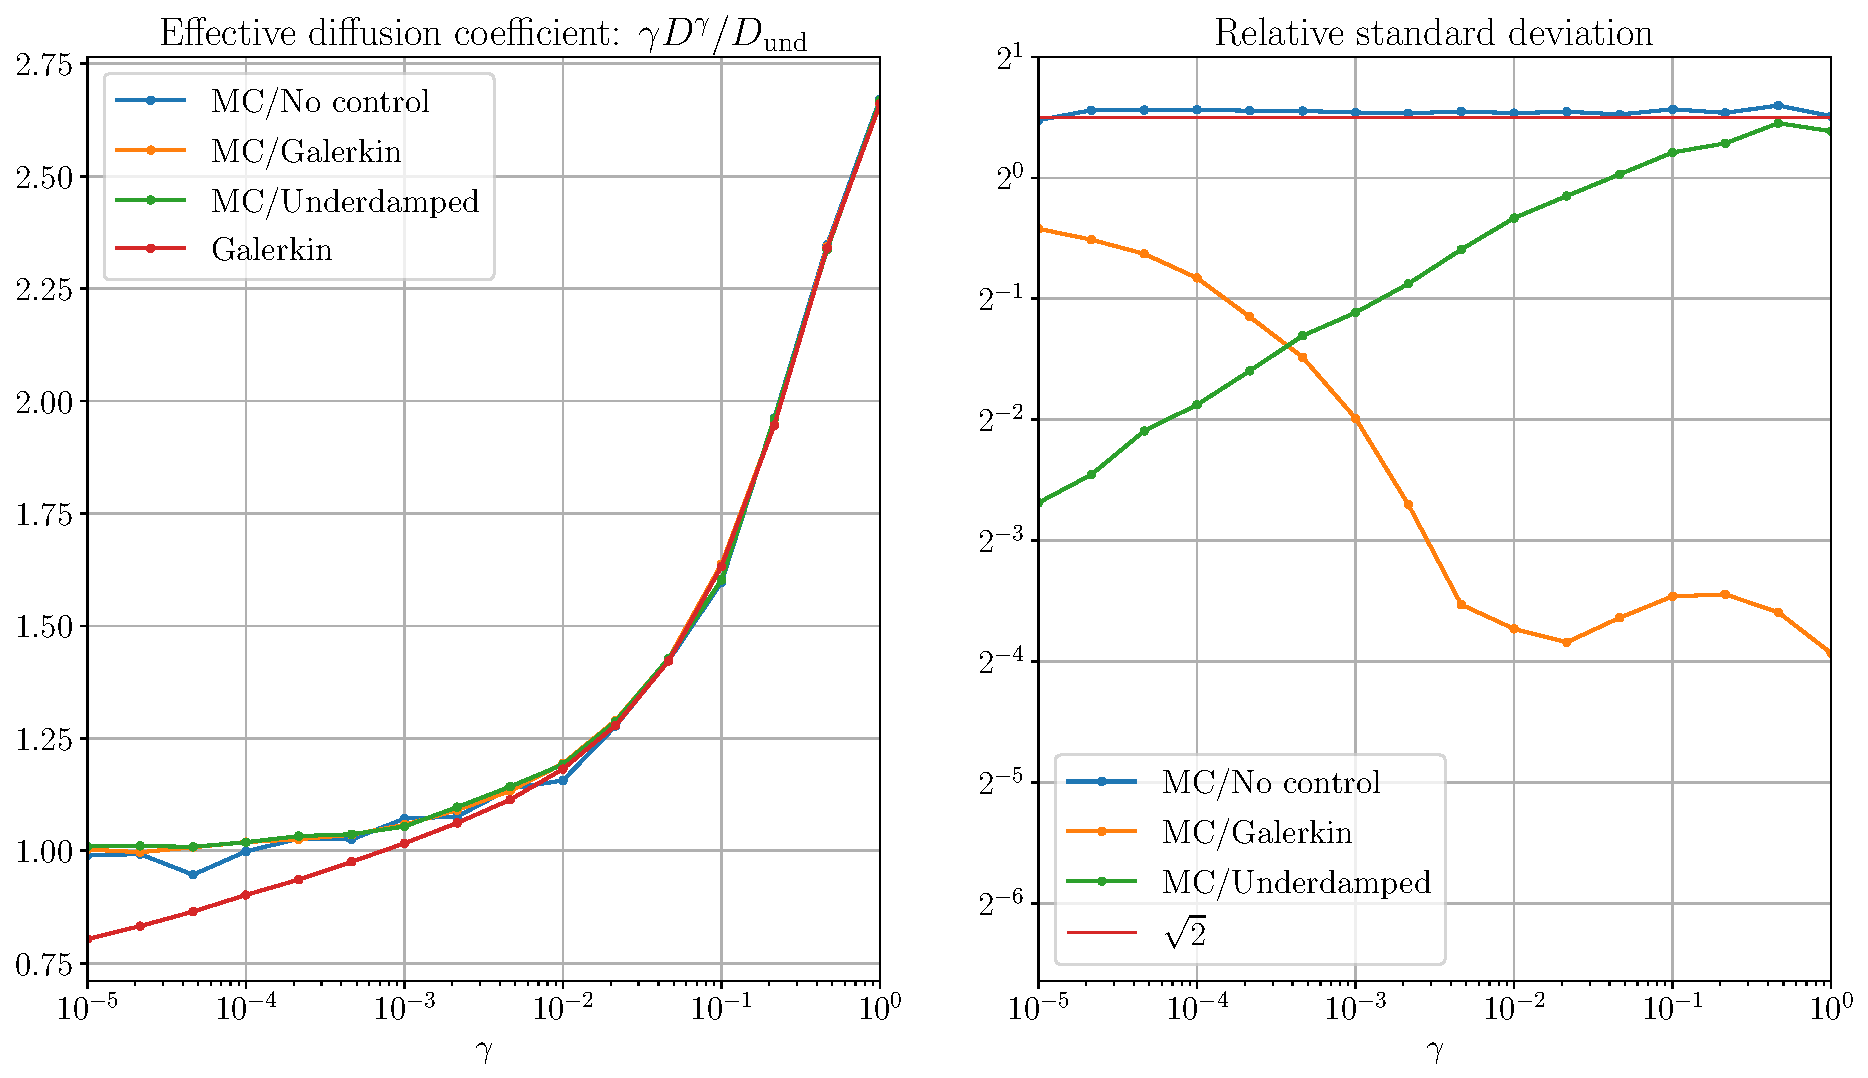
\includegraphics[width=0.99\linewidth]{figures/underdamped_1d.pdf}
    \caption{
        Effective diffusion coefficient and standard deviation of the estimators considered.
        The data labeled ``MC/No control'' correspond to Monte Carlo simulations without a control variate,
        i.e.\ to the estimator $u(T)$ given in~\eqref{eq:simple_estimator}.
        The data labeled ``MC/Galerkin'' and ``MC/Underdamped'' correspond to the improved estimator~\eqref{eq:definition_control_variate},
        with $\psi$ obtained using the approaches of~\cref{sub:galerkin_approach,sub:underdamped_approach},
        respectively.
        Finally, the curve labeled ``Galerkin'' is the approximate diffusion coefficient obtained by the Galerkin method alone,
        which is given by~$\ip*{\widehat \Psi_N}{p}$ in the notation of \cref{sub:galerkin_approach}.
    }%
    \label{fig:effective_diffusion_langevin}
\end{figure}

\Cref{fig:time_bias_variance} illustrates the evolution of the expectation and standard deviation of the estimators~$u(t)$ and~$v(t)$,
estimated from 5000 trajectories,
with respect to the integration time~$t$.
It appears clearly that,
for the value $\gamma = 10^{-3}$ considered,
the improved estimators $v(t)$ obtained using the approaches outlined in \cref{sub:galerkin_approach} and \cref{sub:underdamped_approach}
have a much smaller variance than~$u(t)$ throughout the simulation.
\begin{figure}[ht]
    \centering
    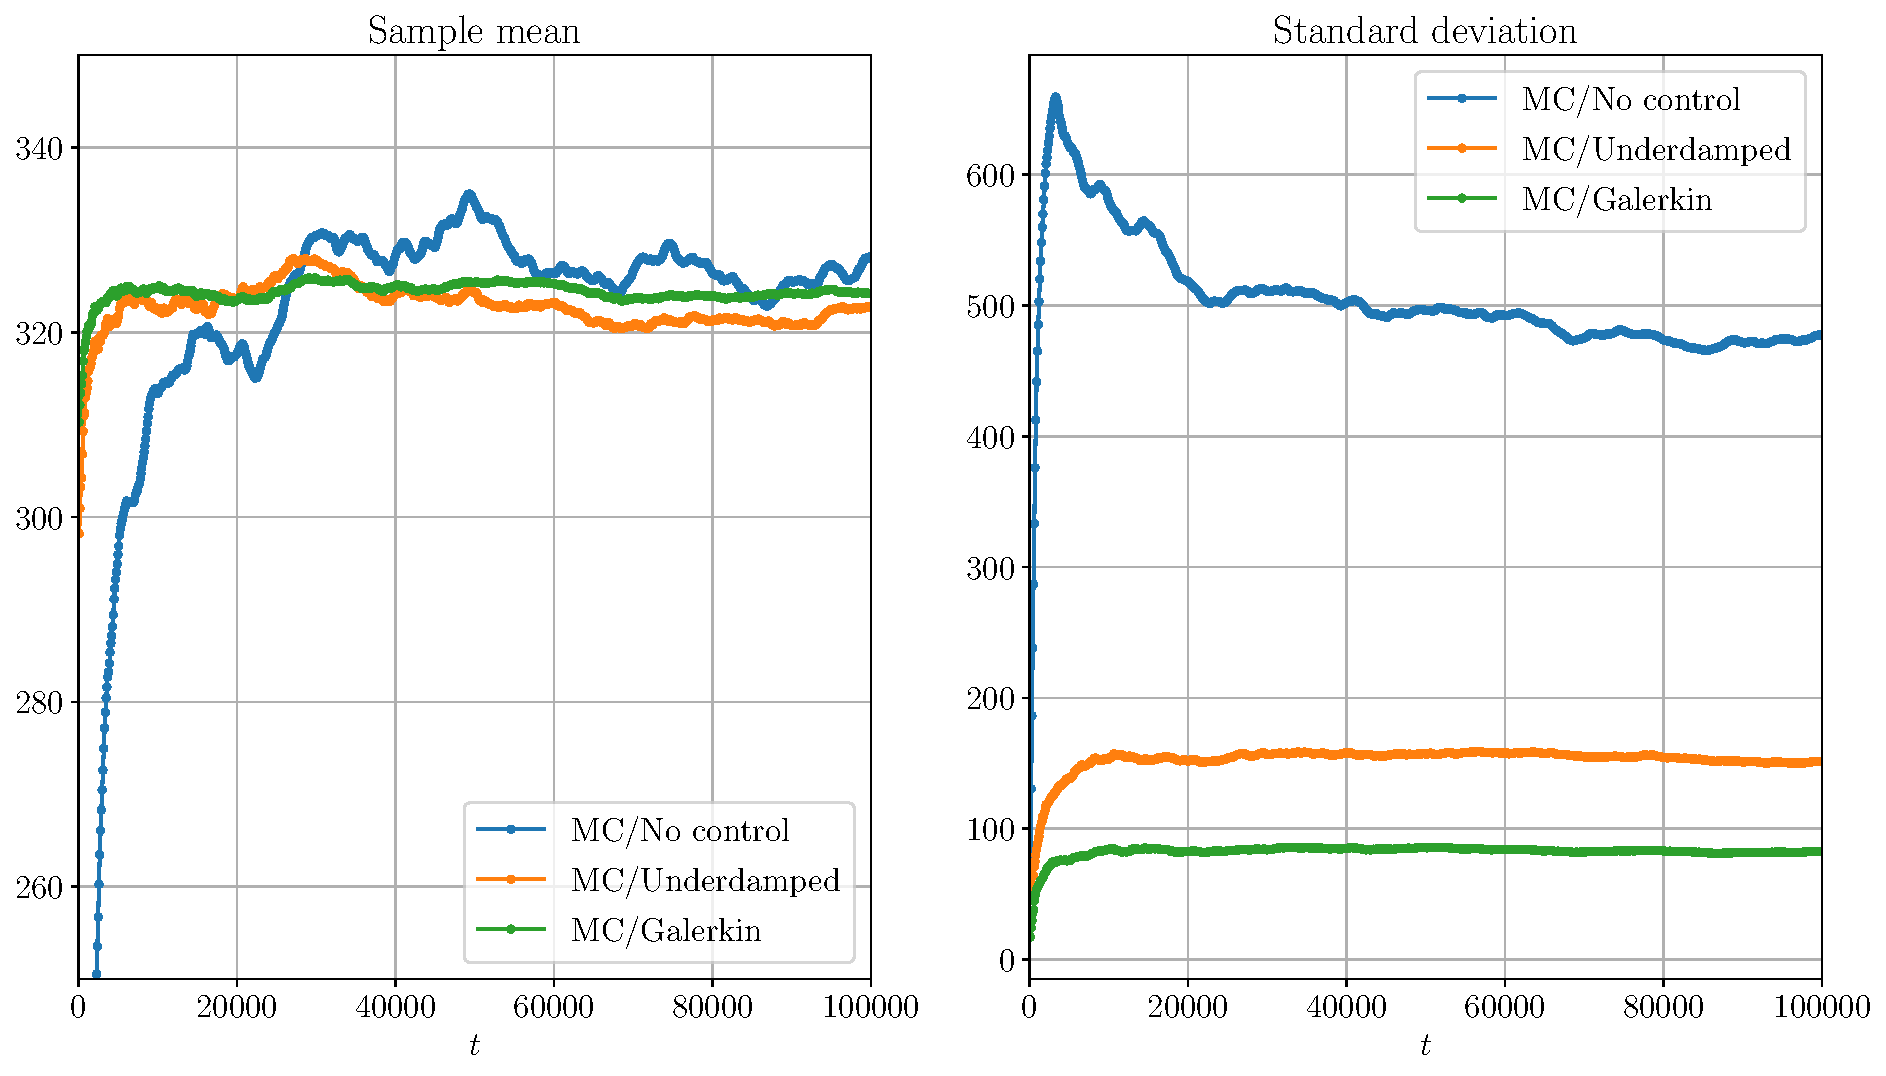
\includegraphics[width=0.99\linewidth]{figures/time.pdf}
    \caption{
        Sample mean and sample standard deviation of the estimators $u(t)$ and $v(t)$,
        for the friction parameter $\gamma = 10^{-3}$.
        The approximate solution to the Poisson equation used for constructing the control variate appearing in $v(t)$ here
        is that given in \cref{sub:underdamped_approach}.
    }%
    \label{fig:time_bias_variance}
\end{figure}

\subsection{Extension to generalized Langevin dynamics}%
\label{sub:generalization_to_generalized_langevin_dynamics}
The variance reduction approach described in \cref{sec:method},
in particular with the control variate constructed from the limiting solution to the Poisson equation as $\gamma \to 0$,
may be extended for calculating the mobility of simple generalized Langevin dynamics in one spatial dimension.
The paradigmatic example dynamics we consider here is the following,
which is studied in~\cite{MR2793823,GPGSUV21}:
\begin{equation}
\label{eq:gle}
\left\{
  \begin{aligned}
      & \d q_t = p_t \, \d t, \\
      & \d p_t = - V'(q_t) \, \d t + \frac{\sqrt{\gamma}}{\nu} \, z_t \, \d t, \\
      & \d z_t = - \frac{\sqrt{\gamma}}{\nu} \, p_t  \, \d t
       -   \frac{1}{\nu^2} \, z_t \, \d t + \sqrt{\frac{2\beta^{-1}}{\nu^2}} \, \d w_t,
  \end{aligned}
\right.
\end{equation}
where $z_t \in \real$.
A functional central limit theorem applies also to this dynamics:
the diffusively rescaled position process $(\varepsilon q_{t/\varepsilon^2})_{t \geq 0}$ converges in distribution,
in the Banach space of continuous functions over a bounded time interval,
to a Brownian motion with prefactor $\sqrt{2 D^{\gamma, \nu}}$.
Like Langevin dynamics, generalized Langevin dynamics are difficult to understand in the underdamped regime,
and in particular there does not exist a rigorous result on the behavior of $D^{\gamma, \nu}$ in the limit as $\gamma \to 0$.
Our goal in this section is to calculate accurately the mobility for the dynamics~\eqref{eq:gle} in the underdamped regime
using a control variate approach similar to that described in~\cref{sec:method},
and to assess in this way the validity of the asymptotic scaling of $D^{\gamma,\nu}$ conjectured in~\cite{GPGSUV21} by means of formal asymptotics.
An application of It\^o's formula gives
\[
    q_T - q_0 = \int_{0}^{T} p_t \, \d t
    = \phi(q_0, p_0, z_0) - \phi(q_T, p_T, z_T) + \sqrt{\frac{2 \beta^{-1}}{\nu^2}} \int_{0}^{T} \partial_z \phi(q_t, p_t, z_t) \, \d t,
\]
where $\phi$ is now the solution to the Poisson equation $- \mathcal L_{\rm GLE} \phi = p$,
with $\mathcal L_{\rm GLE}$ the generator of~\eqref{eq:gle}.
This suggests using the following estimator for the mobility:
\begin{subequations}
\begin{equation}
    \label{eq:improved_estimator_gle}
    v(T) = d[\psi] + \frac{1}{2T} \left( \abs*{q_T - q_0}^2 - \abs{\xi_T}^2\right),
    \qquad d[\psi] := \sqrt{\frac{2 \beta^{-1}}{\nu^2}} \int \abs{\partial_z \psi}^2 \, \d \mu_{\rm GLE}.
\end{equation}
where
\begin{align}
    \label{eq:definition_control_variate_gle}
    \xi_T = \psi(q_0, p_0, z_0) - \psi(q_T, p_T, z_T) + \sqrt{\frac{2 \beta^{-1}}{\nu^2}} \int_{0}^{T} \partial_z \psi(q_t, p_t, z_t) \, \d w_t,
\end{align}
\end{subequations}
for an approximate solution $\psi$ to the Poisson equation,
and with $\mu_{\rm GLE}$ the invariant probability distribution of~\eqref{eq:gle}:
\[
    \mu_{\rm GLE}(\d q \, \d p \, \d z) \propto \exp \biggl( - \beta \left( H(q,p) + \frac{z^2}{2} \right) \biggr) \, \d q \, \d p \, \d z.
\]

In~\cite{GPGSUV21},
we employ an asymptotic expansion of the form
\(
    \phi = \gamma^{-1} \phi_0 + \gamma^{-1/2} \phi_1 + \gamma^{-1} \phi_2 + \dotsb
\)
in order to study the underdamped limit
and we derive expressions for $\phi_0$ and $\phi_1$
which enable to show formally that $D^{\gamma, \nu}$ behaves as $\gamma^{-1}$ in the limit as $\gamma \to 0$,
with a prefactor that can be calculated efficiently and is different from $D_{\rm und}$.
Although the assumed asymptotic expansion is shown to be invalid in~\cite{GPGSUV21}
because $\mathcal L_{\rm GLE} \phi_1 \notin \lp{2}{\mu}$,
our numerical results in this section demonstrate that this expansion can still be leveraged for constructing an efficient control variate $\xi_T$ in~\eqref{eq:definition_control_variate_gle}.
Specifically,
we obtain a considerable reduction in variance by choosing in~\eqref{eq:definition_control_variate_gle} as $\psi = \gamma^{-1} \phi_0 + \gamma^{-1/2} \phi_1$.
We refer to~\cite[Section~4.3.2] {GPGSUV21} for the expressions of the functions $\phi_0$ and $\phi_1$.

\Cref{fig:effective_diffusion_time_gle} illustrates the evolution of $\expect u(t)$ and $\expect v(t)$ with respect to time,
for a value of~$\nu = 2$ that is sufficiently large to observe a different asymptotic behavior than that of standard Langevin dynamics.
These expectations are estimated from 5000 independent trajectories,
and the associated $[m - 3 s, m + 3 s]$ confidence intervals (corresponding to a confidence of approximately $99.7\%$ assuming Gaussianity) are depicted,
where $m$ and $s$ are the sample mean and sample standard deviation.
It is evident from the figures that the control variate enables considerable improvements,
both in terms of bias and variance.
Furthermore, we observe that the effective diffusion coefficient for $\gamma = 10^{-5}$
is in very good agreement with the limit conjectured in~\cite{GPGSUV21}.
The evolution of the effective diffusion with respect to $\gamma$ is presented in~\cref{fig:effective_diffusion_gle}.
\begin{figure}[ht]
    \centering
    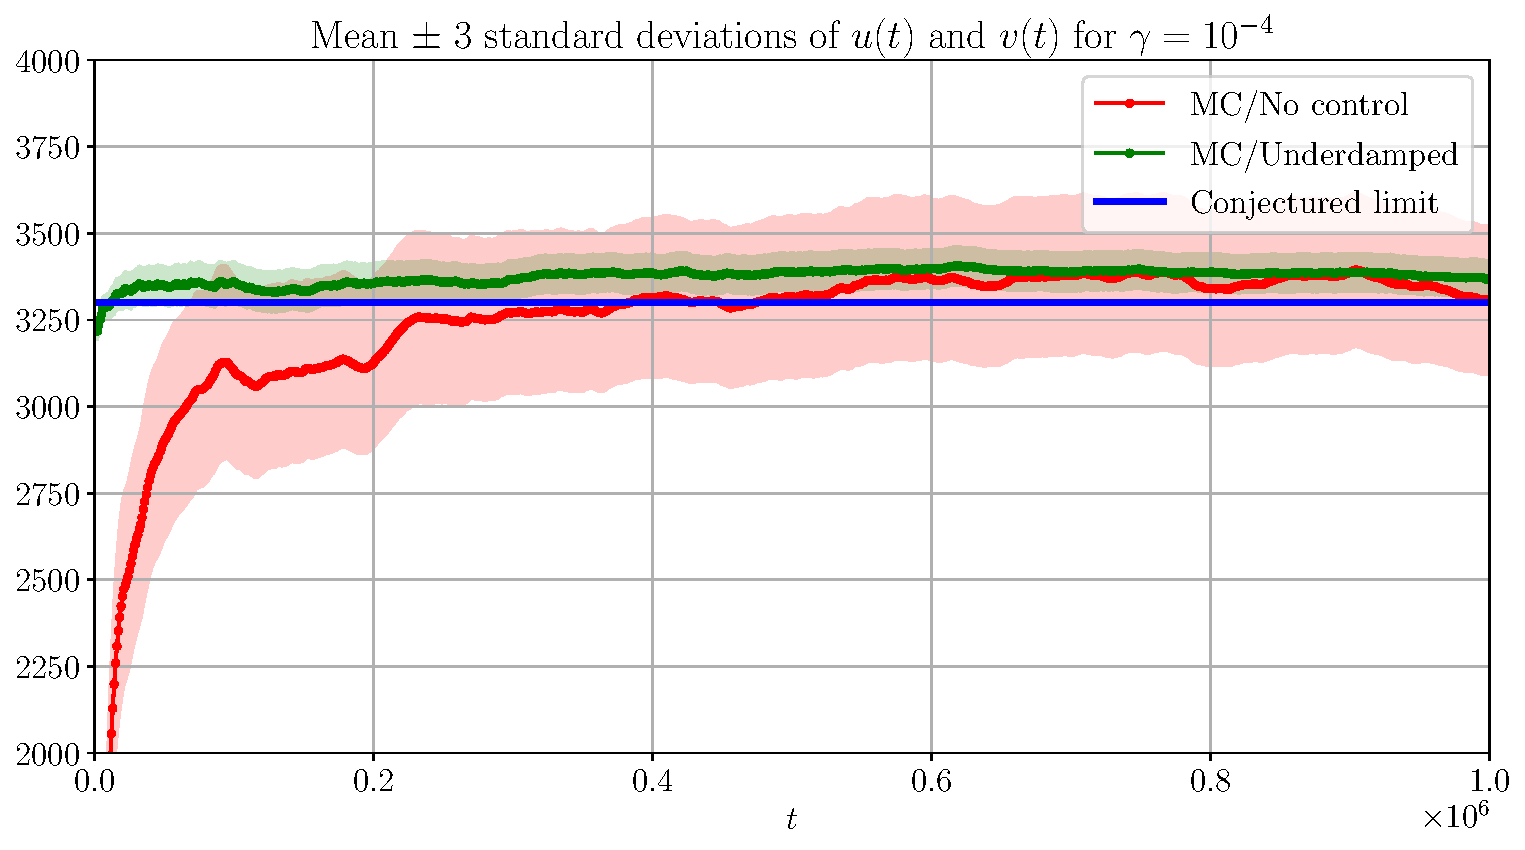
\includegraphics[width=0.495\linewidth]{figures/time-gle-4.pdf}
    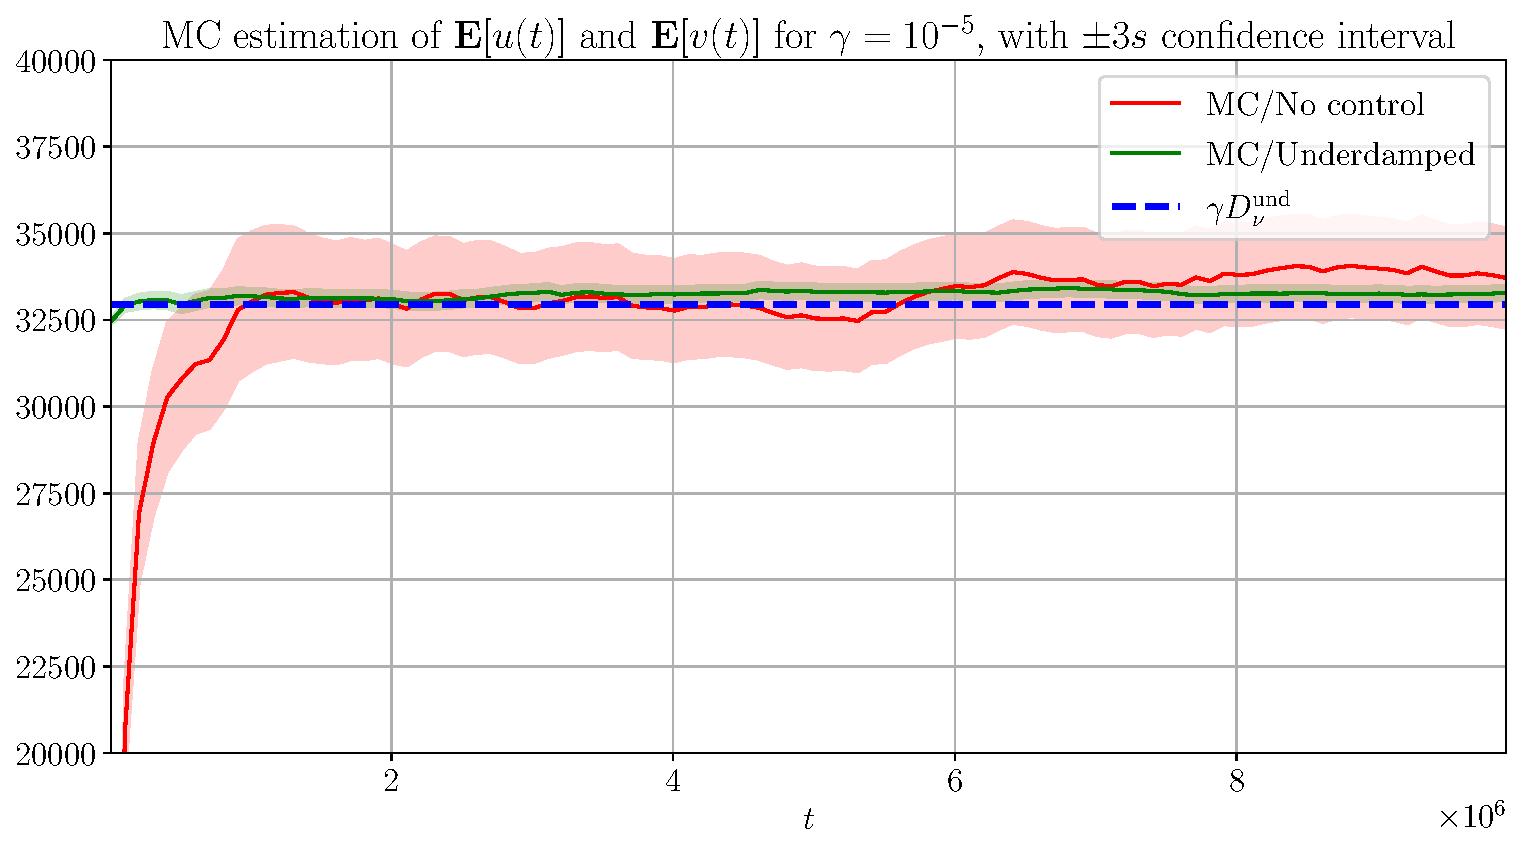
\includegraphics[width=0.495\linewidth]{figures/time-gle-5.pdf}
    \caption{%
        Expectations of the naive~\eqref{eq:simple_estimator} and improved~\eqref{eq:improved_estimator_gle} estimators for generalized Langevin dynamics
        and associated ``$m \pm 3 s$'' confidence intervals,
        estimated from $5000$ trajectories.
        The left panel is for $\gamma = 10^{-4}$ and the right panel is for $\gamma = 10^{-5}$.
    }
    \label{fig:effective_diffusion_time_gle}
\end{figure}
\begin{figure}[ht]
    \centering
    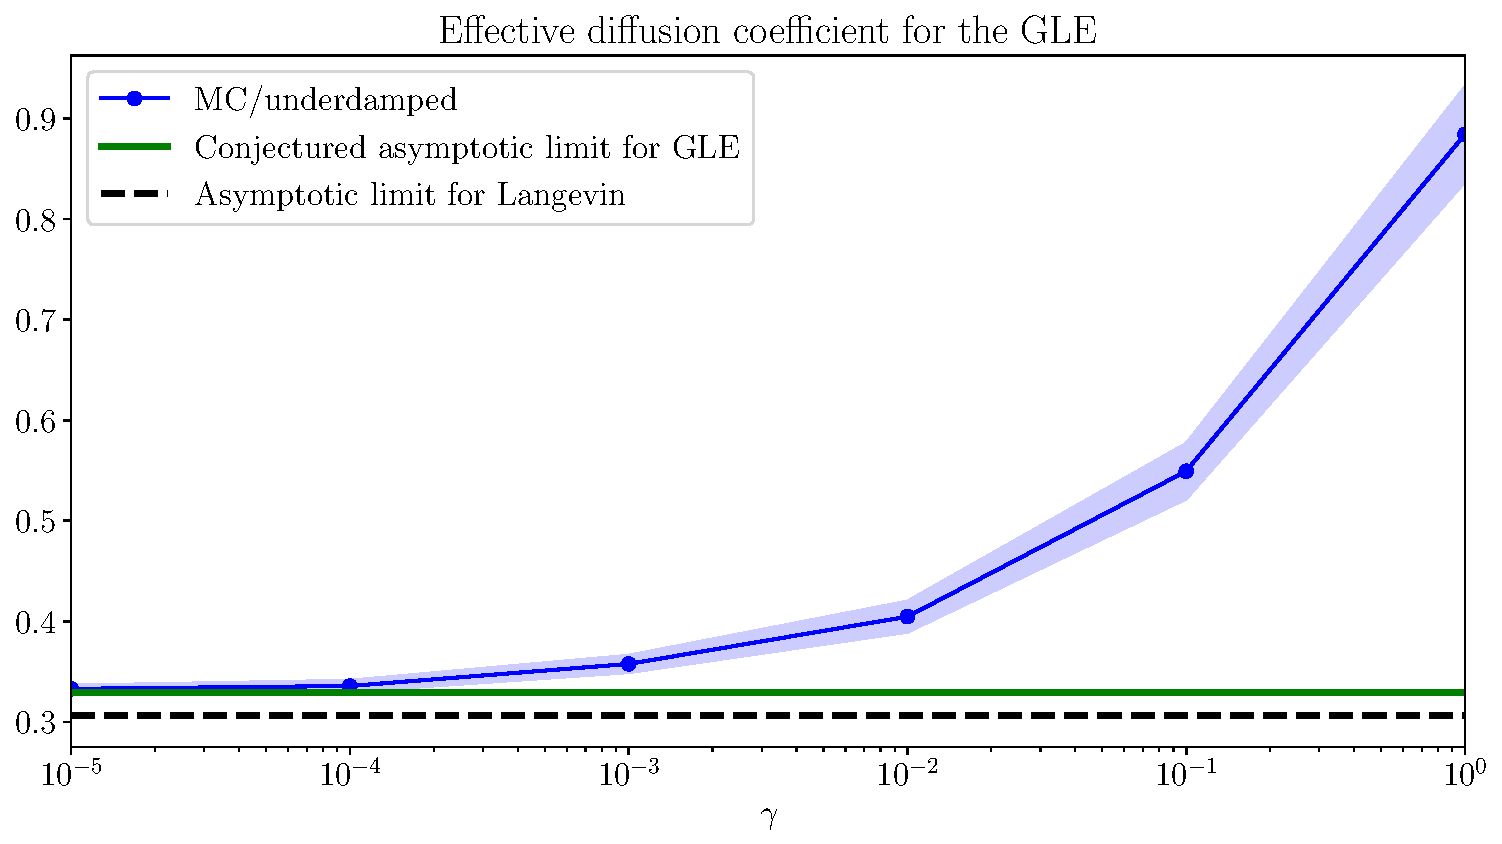
\includegraphics[width=0.75\linewidth]{figures/mobility_gle.pdf}
    \caption{%
        Expectation and ``$m \pm 3 s$'' confidence intervals for $v(T)$ in the underdamped limit,
        in the case of generalized Langevin dynamics with $\nu = 2$.
        Since $T$ scales as $1/\gamma$ with a large prefactor,
        it is expected that $\expect v(T) \approx D^{\gamma,\nu}$.
    }
    \label{fig:effective_diffusion_gle}
\end{figure}


% An alternative viewpoint on the control variate approach presented in \cref{sub:galerkin_approach} is that
% Monte Carlo simulation is employed in order to refine estimates obtained by Fourier/Hermite spectral method for the Poisson equation~\eqref{eq:poisson_equation}.

\section{Application to Langevin dynamics in two dimensions}%
\label{sec:applications_2d}%
The approaches employed in \cref{sec:application_to_one_dimensional_langevin_type_dynamics} for constructing an approximate solution to the Poisson equation~\eqref{eq:poisson_equation}
do not generalize well to the multi-dimensional setting for non-separable potentials.
On one hand, Galerkin methods for the Poisson equation suffer from the curse of dimensionality and,
on the other hand, the behavior of the solution to the Poisson equation is not well understood in the underdamped limit.
In this section we discuss alternative approaches.
We consider in this work a non-separable potential even simpler than~\eqref{eq:potential_julien}:
\begin{align}
    \label{eq:potential_simple}
    V(q) =  \mathcal V(q_1) + \mathcal V(q_2) + \delta \mathcal W(q_1, q_2) := - \cos(q_1) - \cos(q_2) - \delta \cos(q_1) \cos(q_2).
\end{align}
In view of the symmetry of this potential,
the diffusion tensor $\mat D^{\gamma}$ is a multiple of the identity.
Indeed, it is clear that $D^{\gamma}_{11} = D^{\gamma}_{22}$,
and $D^{\gamma}_{12} = 0$ because if $\bigl((q_t, p_t)\bigr)_{t \geq 0}$ is a weak solution to~\eqref{eq:langevin},
then so is $\bigl((R \vect q_t, R \vect p_t)\bigr)_{t \geq 0}$ with $R: \real^2 \to \real^2; (x_1, x_2) \mapsto (x_1, -x_2)$,
and thus
\begin{align*}
    D^{\gamma}_{12}
    &= \frac{1}{2T} \lim_{\tau \to \infty}
    \expect \left[ \bigl(\vect e^\t (\vect q_{\tau} - \vect q_0)\bigr) \bigl(\vect f^\t (\vect q_{\tau} - \vect q_0)\bigr) \right] \\
    &= - \frac{1}{2T} \lim_{\tau \to \infty}
    \expect \left[ \bigl(\vect e^\t (R \vect q_{\tau} - R \vect q_0)\bigr) \bigl(\vect f^\t (R \vect q_{\tau} - R \vect q_0)\bigr) \right]
    = - D^{\gamma}_{12}
\end{align*}
with $\vect e = (1, 0)^\t$ and $\vect f = (0, 1)^\t$,
and where the first and last equalities follow from the definition~\eqref{eq:einsteins_formula} of the effective diffusion coefficient.
Note that this can also be shown at the level of~\eqref{eq:effective_diffusion_poisson}.
Since $\mat D^{\gamma}$ is a multiple of the identity,
we can focus on estimating $D^{\gamma}_{\vect e}$ only for the unit vector $\vect e_1 = (1, 0)^\t$,
which simplifies the discussion.
Let $\phi_\delta(q, p)$ denote the solution to the Poisson equation $- \mathcal L^{\delta} \phi_\delta = p_1$,
where the generator~$\mathcal L^{\delta}$ of the dynamics now reads
\begin{align}
    \label{eq:generator}
    \mathcal L^{\delta} = \mathcal L_0 + \delta \mathcal L_1
    := L_1 + L_2
    - \delta \grad \mathcal W \cdot \grad_{\vect p},
\end{align}
with $L_i = p_i \partial_{q_i} - \mathcal V'(q_i) \, \partial_{p_i} + \gamma \left(- p_i \partial_{p_i} + \beta^{-1} \partial^2_{p_i} \right)$,
for $i \in \{1, 2\}$.
Notice that $\phi_\delta(q, p) = \phi(q_1, p_1)$ when $\delta = 0$,
where $\phi$ is the solution to the one-dimensional Poisson equation $-L_1 \phi(q_1, p_1) = p_1$.
In other words, it holds $\phi_0 = \phi \otimes 1$,
where for two functions $f_1: \torus \times \real \rightarrow \real$ and $f_2: \torus \times \real \rightarrow \real$
the notation $f_1 \otimes f_2$ denotes the function $(\vect q, \vect p) \mapsto f_1(q_1,p_1) \, f_2(q_2,p_2)$.
For small $\delta$, it is natural to use $\phi_0$, or an approximation thereof,
as the function $\psi_{\vect e}$ in the definition of the control variate~\eqref{eq:definition_control_variate}.
Note that $d[\psi_{\vect e}]$ in~\eqref{eq:definition_control_variate} is with this approach an average with respect to the invariant distribution of the non-separable dynamics,
which we denote by $\mu_{\delta}$ to emphasize its dependence on $\delta$.
% In particular $d[\psi_{\vect e}]$ takes different values than in the one-dimensional setting:
% denoting by $\psi$ an approximation of $\phi$,
% and assuming that the approximate solution to the Poisson equation for the multi-dimensional dynamics,
% used in the control variate~\eqref{eq:definition_control_variate},
% is given by $\psi_{\vect e}(q,p) = \psi(q_1, p_1)$,
% we have
% \[
%     d[\psi_{\vect e}]
%     = \int_{\torus^d \times \real^d} \abs{\grad_{\vect p} \psi_{\vect e}}^2 \, \d \mu_{\delta}
%     = \int_{\torus^d \times \real^d} \abs{\partial_p \psi}^2 \, \d \mu_{\delta}.
% \]

\Cref{fig:time_bias_variance_2d} depicts the behaviour of the mobility with respect to $\gamma$ for different values of $\delta$.
It appears clearly from the figure that the mobility behaves as $\gamma^{-\sigma}$ for $\sigma \in (0, 1]$ in the underdamped regime,
with an exponent $\sigma$ that decreases as $\delta$ increases (at least for sufficiently small values of~$\delta$).
The variance of the estimators obtained using the approach described above,
where $\psi_{\vect e}$ is constructed from an approximate solution to the Poisson equation in the one-dimensional setting,
is presented in~\cref{fig:time_bias_deviation_2d}.
We observe that, unless $\delta = 0$ in which case we recover the one-dimensional case,
there is for every $\delta > 0$ and for each of the two choices of $\psi_{\vect e}$,
a threshold value of $\gamma$ below which the control variate ceases to be useful.
This result establishes that~$\phi_\delta \to \phi_0$ in the limit as~$\delta \to 0$.
\begin{proposition}
    Let $\phi_{\delta}$ and $\phi_0$ denote the solutions to the Poisson equation $- \mathcal L^{\delta} \phi_{\delta} = p_1$
    and its separable counterpart $- \mathcal L_0 \phi_0 = p_1$,
    in $L^2_0(\mu_{\delta})$ and $L^2_0(\mu_0)$ respectively.
    Then there exists $C$ independent of $\delta$ and $\gamma$ such that 
    \begin{equation}
        \label{eq:convergence_mobility_delta}
        \norm*{\grad_{\vect p} \phi_\delta - \grad_{\vect p} \phi_0}[L^2(\mu_{\delta})]
        = C \delta \gamma^{-2}
    \end{equation}
    % and denote
    % \[
    %     d^{\delta}_{\phi_\delta} = \int \abs{\grad \phi_\delta}^2 \, \d \mu_{\delta},
    %     \qquad
    %     d^{\delta}_{\phi_0} = \int \abs{\grad \phi_0}^2 \, \d \mu_{\delta}.
    % \]
\end{proposition}
\begin{proof}
    As mentioned after~\eqref{eq:generator},
    it holds that $\phi_0 = \phi \otimes 1$ with $\phi$ the solution to the Poisson equation in spatial dimension 1 and potential $\mathcal V$.
    We consider the decomposition~\eqref{eq:generator} of the generator and note that
    \begin{equation}
        \label{eq:remainder_expansion}
        \mathcal L^{\delta}(\phi_\delta - \phi_0)
        = - \delta \, \mathcal L_1 \phi_0
        = \delta \, \partial_{q_1} \mathcal W(q_1, q_2) \, \partial_{p_1} \phi(q_1, p_1).
    \end{equation}
    Let $\phi_0^{\delta}$ denote the $L^2(\mu_{\delta})$ orthogonal projection of $\phi_0$ onto $L^2_0(\mu_{\delta})$.
    Taking the $L^2(\mu_{\delta})$ inner product of both sides of~\eqref{eq:remainder_expansion} with $(\phi_\delta - \phi_0^{\delta})$,
    we obtain
    \begin{align*}
        \gamma \beta^{-1} \norm*{\grad_{\vect p} \phi_\delta - \grad_{\vect p} \phi_0^{\delta}}[L^2(\mu_{\delta})]^2
        &\leq \delta \norm*{\partial_{q_1} \mathcal W(q_1, q_2) \, \partial_{p_1} \phi(q_1, p_1)}[L^2(\mu_{\delta})] \norm*{\phi_\delta - \phi_0^{\delta}}[L^2(\mu_{\delta})] \\
        &\leq C \delta \norm*{\partial_{p_1} \phi(q_1, p_1)}[L^2(\mu_{\delta})] \norm*{\phi_\delta - \phi_0^{\delta}}[L^2(\mu_{\delta})]
    \end{align*}
    for all $(\gamma, \delta) \in (0, \infty) \times [-1, 1]$. 
    Throughout this proof, $C$ denotes a constant independent of $\gamma$ and $\delta$,
    whose value can change from occurrence to occurrence.
    Since the $\vect q$ marginal of $\mu_{\delta}$ is equivalent to the Lebesgue measure on $\torus^d$,
    with a smooth positive density that can be bounded, both from below by a strictly positive constant and from above, independently of $\delta$ for all $\delta \in [-1, 1]$,
    there exists a constant $C_P > 0$ such that $\mu_{\delta}$ satisfies the Poincaré inequality uniformly: 
    \begin{align}
        \label{eq:poincare_for_mudelta}
        \forall \delta \in [-1, 1], \qquad
        \norm*{\phi_\delta - \phi_0^{\delta}}[L^2(\mu_{\delta})] \leq C_P \norm*{\grad_{\vect p} \phi_\delta - \grad_{\vect p} \phi_0^{\delta}}[L^2(\mu_{\delta})].
    \end{align}
    Therefore, it holds that
    \begin{equation}
        \label{eq:bound_gradient_of_difference}
        \gamma \beta^{-1} \norm*{\grad_{\vect p} \phi_\delta - \grad_{\vect p} \phi_0^{\delta}}[L^2(\mu_{\delta})]
        \leq C \delta \norm*{\grad_{\vect p} \phi_0^{\delta}}[L^2(\mu_{\delta})]
        = C \delta \norm*{\grad_{\vect p} \phi_0}[L^2(\mu_{\delta})].
    \end{equation}
    Now since $\phi_0$ solves $- \mathcal L_0 \phi_0 = p_1$,
    we have
    \[
        \gamma \beta^{-1} \norm{\grad_{\vect p} \phi_0}[L^2(\mu_0)]^2
        = - \ip{\phi_0}{\mathcal L \phi_0}[L^2(\mu_0)] = \ip{\phi_0}{p}[L^2(\mu_0)] 
        \leq \beta^{-1/2} \norm{\phi_0}[L^2(\mu_0)] 
        \leq C_P \beta^{-1/2} \norm{\grad_{\vect p} \phi_0}
    \]
    and so we deduce~\eqref{eq:convergence_mobility_delta}.
\end{proof}
\begin{remark}
    which gives the result since $\grad_{\vect p} \phi_0^{\delta} = \grad_{\vect p} \phi_0$.
    Let $\phi_0^{\delta}$ denote the $L^2(\mu_{\delta})$ orthogonal projection of $\phi_0$ onto $L^2_0(\mu_{\delta})$.
    It follows from~\eqref{eq:remainder_expansion} that
    \[
        \norm*{\phi_\delta - \phi_0^{\delta}}[L^2(\mu_{\delta})]
        \leq \delta \norm*{(\mathcal L^{\delta})^{-1}} [\mathcal B\left(L^2_0(\mu_{\delta})\right)] \norm{\partial_{q_1} \mathcal W(q_1, q_2) \, \partial_{p_1} \phi(q_1, p_1)}[L^2(\mu_{\delta})].
    \]
    The resolvent norm on the right-hand side is uniformly bounded from above for $\delta \in [1, 1]$ using standard results,
    and it is clear that
    \(
        c_1 \norm{\dummy}[L^2(\mu_{\delta})] \leq \norm{\dummy}[L^2(\mu_0)] \leq c_2 \norm{\dummy}[L^2(\mu_{\delta})]
    \)
    for appropriate constants $c_1, c_2 > 0$ and all $\delta \in [-1, 1]$.
    Therefore, we have
    \begin{equation}
        \label{eq:intermediate_expansion_delta}
        \forall (\gamma, \delta) \in (0, 1] \times [-1, 1], \qquad
        \norm*{\phi_\delta - \phi_0^{\delta}}[L^2(\mu_{\delta})]
        \leq C \delta \gamma^{-1} \, \norm{\partial_{p_1} \phi(q_1, p_1)}[L^2(\mu_{0})]
        \leq C \delta \gamma^{-2},
    \end{equation}
    because the norm on the right-hand side of the first inequality is the mobility of one-dimensional Langevin dynamics,
    which scales as $\bigo{\gamma^{-1}}$.
    Now since $\d \mu_{\delta} / \d \mu_0  = 1 + \delta f_{\delta}(q_1, q_2)$ for some appropriate function $f_{\delta}$ that is uniformly bounded from above over $(\delta, q_1, q_2) \in [-1, 1] \times \torus \times \torus$,
    we deduce
    \[
        \norm*{\phi_0^\delta - \phi_0} [L^2(\mu_\delta)]
        = \abs{ \int \phi_0 \, \d \mu_{\delta} }
        = \abs{ \int \phi_0 \,\bigl( 1 + \delta f_{\delta}(q_1, q_2) \bigr)\d \mu_{0}}
        \leq C \delta \norm{\phi_0}[L^2(\mu_0)] \leq C \delta \gamma^{-1},
    \]
    which combined with~\eqref{eq:intermediate_expansion_delta} gives~\eqref{eq:convergence_solution_delta}.
\end{remark}
\begin{remark}
    Combining~\eqref{eq:bound_gradient_of_difference} with the upper bound in~\cref{proposition:asymptotic_variance},
    we deduce that,
    assuming the exact solution to the Poisson equation in one spatial dimension is employed for constructing the control variate,
    the asymptotic variance is bounded from above by $C \delta^2 \gamma^{-4}$,
    which suggests a scaling as $\delta/\gamma$ for the asymptotic relative standard deviation
    (relative to the limit as $\delta \to 0$).
    \textcolor{red}
    {This still needs improvements. Can we show, for example, that if we take $\delta \propto 1/\gamma$,
    the relative standard deviation remains bounded from above as $\gamma \to 0$?}
\end{remark}
\begin{figure}[ht]
    \centering
    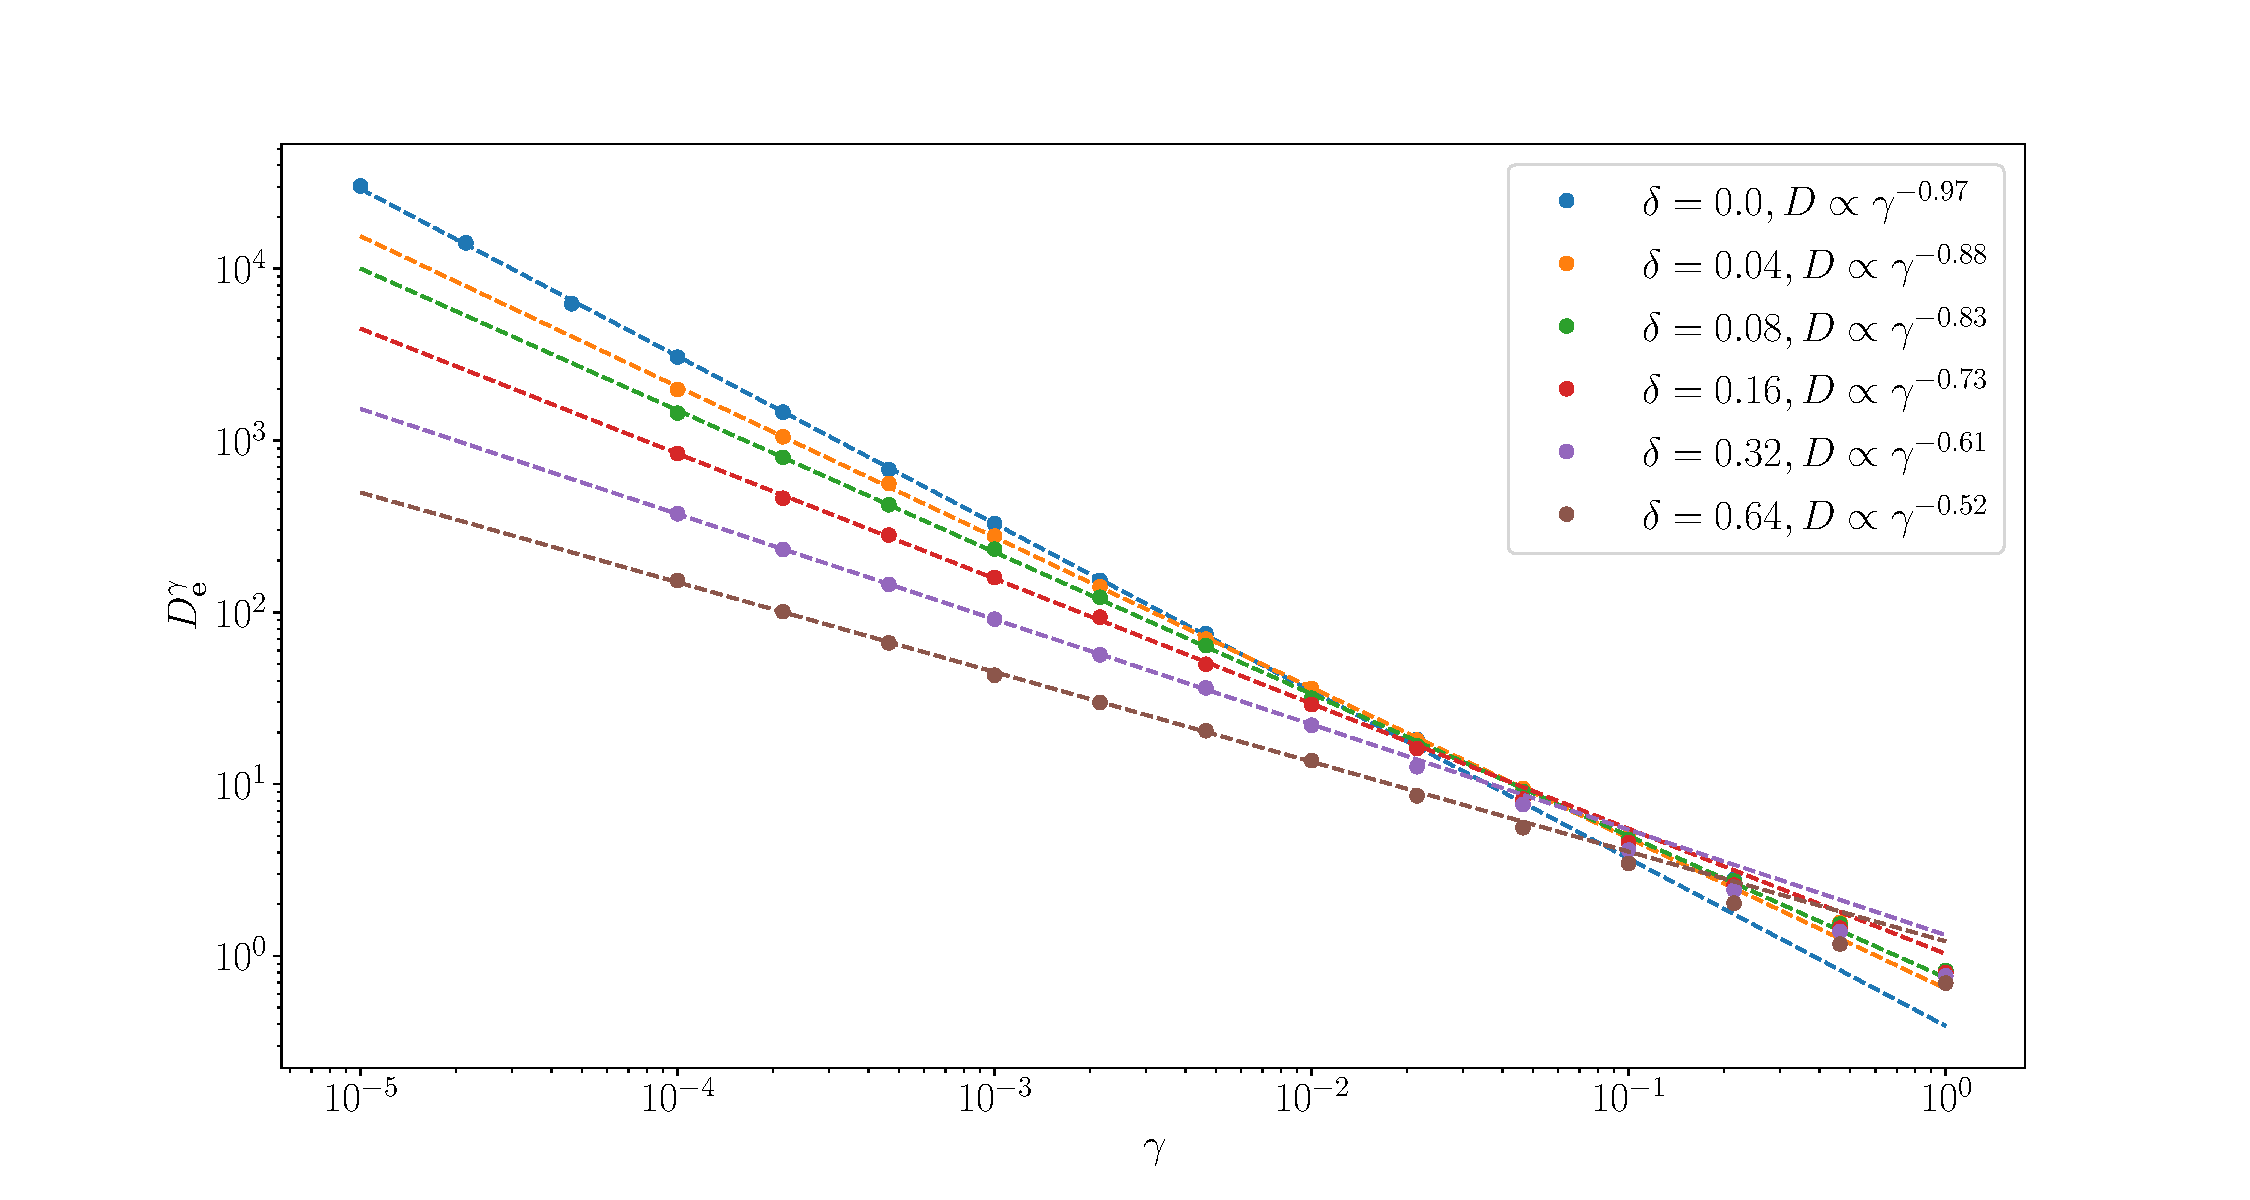
\includegraphics[width=0.99\linewidth]{figures/diffusion.pdf}
    \caption{
        Effective diffusion coefficient as a function of $\gamma$,
        for different values of $\delta$.
    }%
    \label{fig:time_bias_variance_2d}
\end{figure}

\begin{figure}[ht]
    \centering
    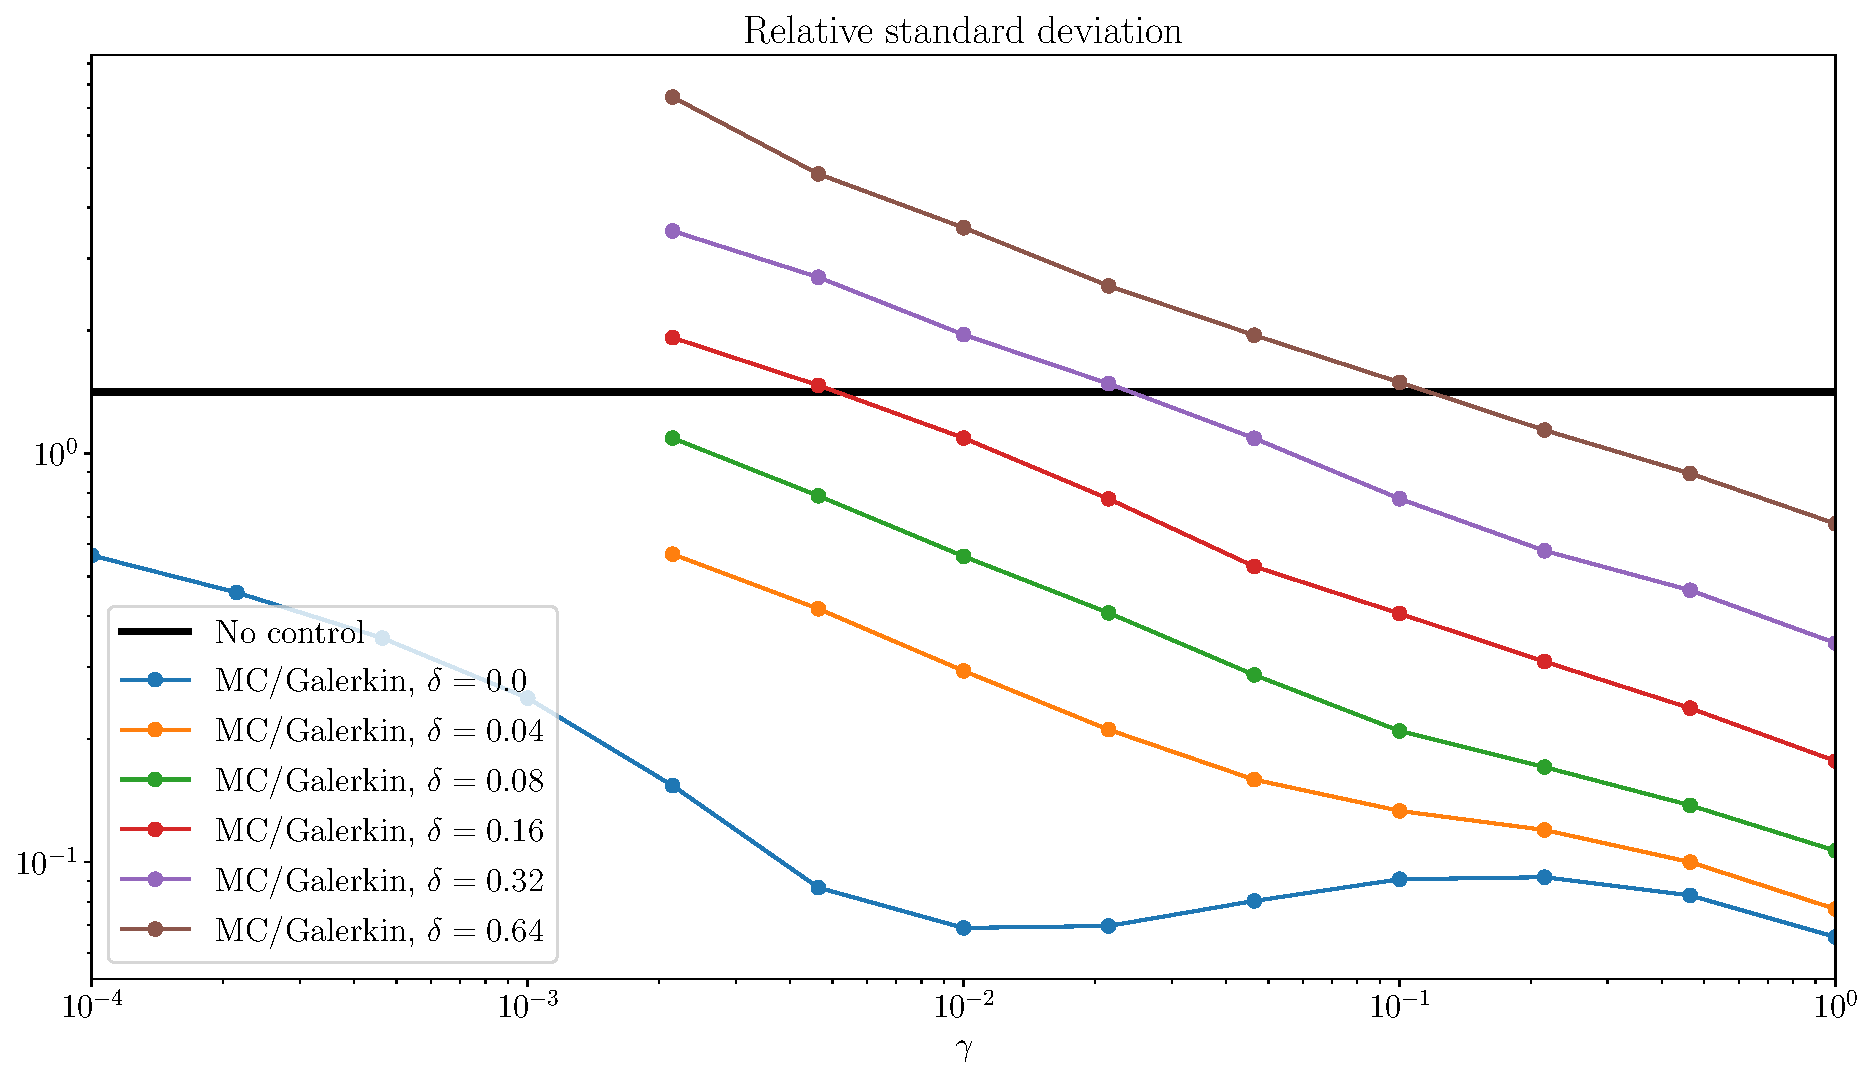
\includegraphics[width=0.49\linewidth]{figures/var-delta-galerkin.pdf}
    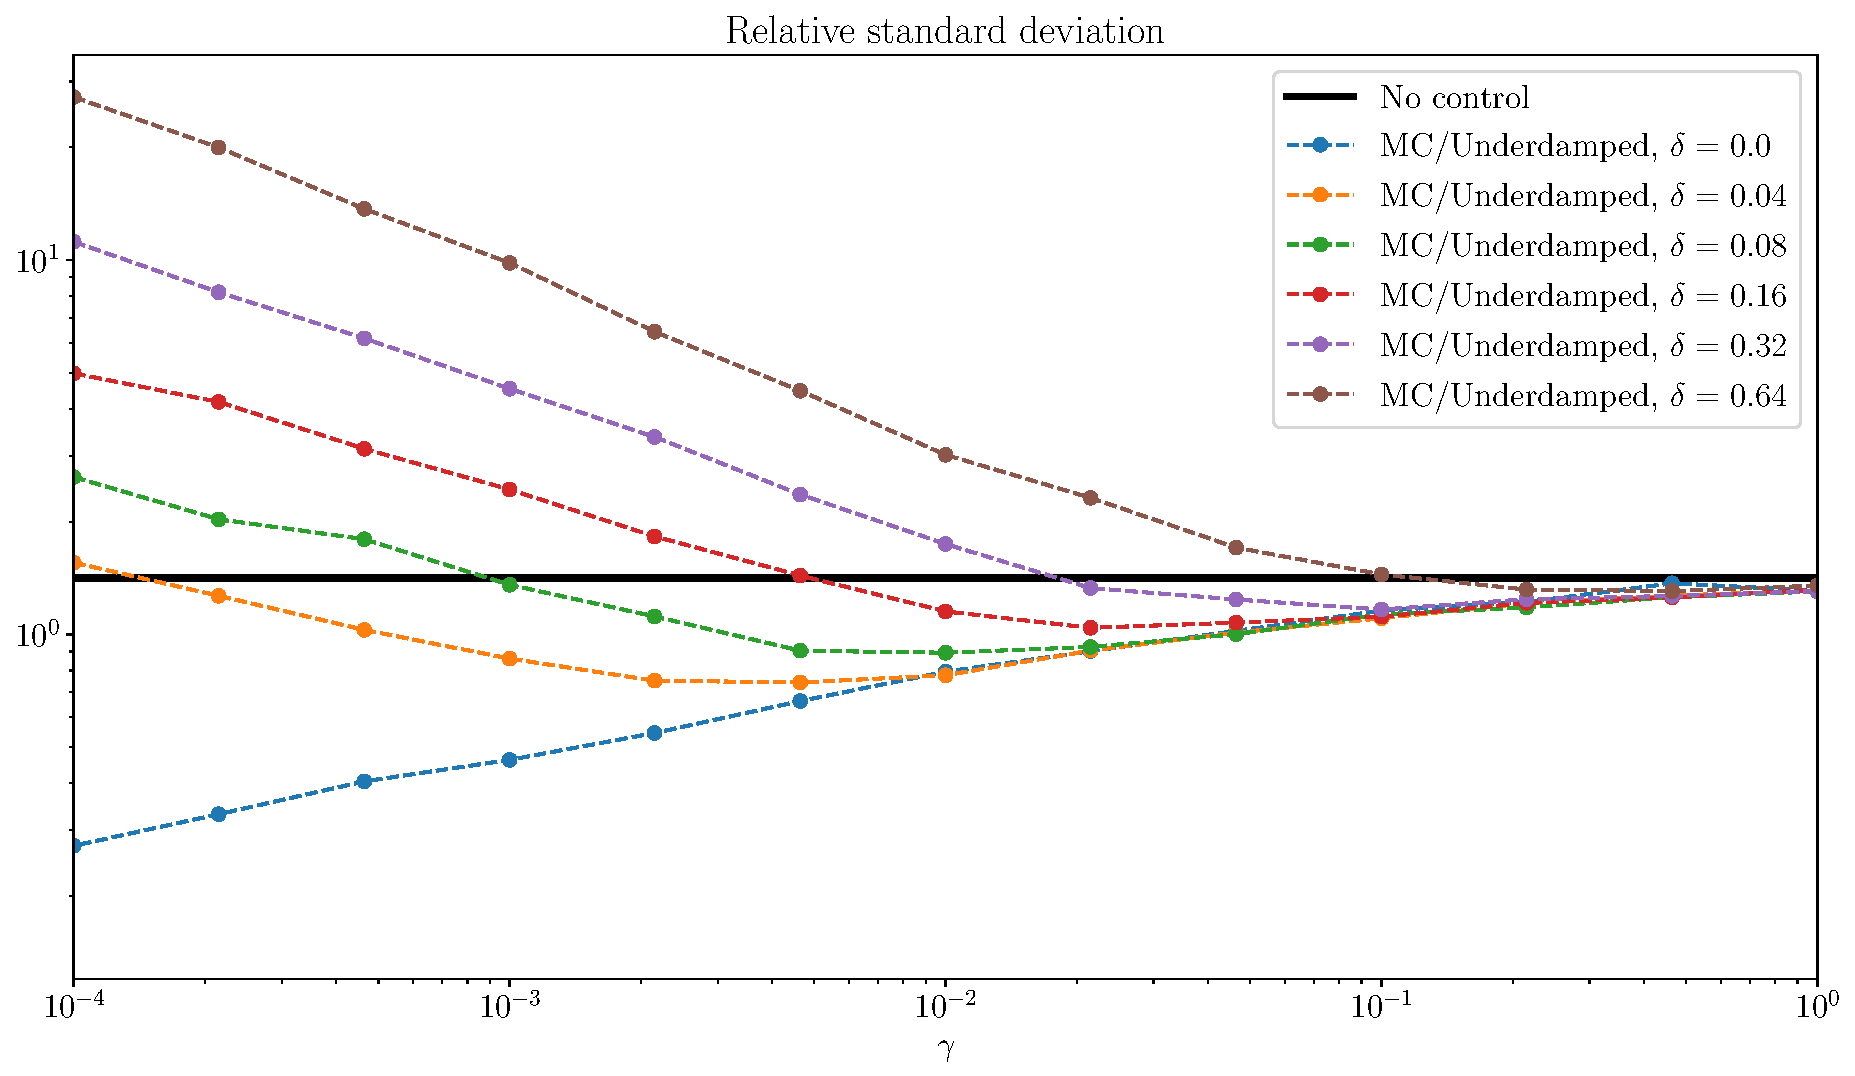
\includegraphics[width=0.49\linewidth]{figures/var-delta-underdamped.pdf}
    \caption{
        Relative standard deviation of the estimator $v(T)$ for two-dimensional Langevin dynamics,
        when the approximate solution to the Poisson equation is constructed by tensorization from the solution of the one-dimensional equation.
    }%
    \label{fig:time_bias_deviation_2d}
\end{figure}

\section{Conclusions and perspectives for future work}%
\label{sec:conclusions_and_perspectives_for_future_work}
In this note,
we show how techniques based on control variates can be employed for improving estimators of the mobility of Langevin dynamics based on Einstein's formula.
The control variate approach we propose requires the knowledge of an approximate solution of a Poisson equation involving the generator of the dynamics.
We obtain general bounds on the bias and variance of the improved estimator in terms of the error on the solution to this equation,
and we study several practical approaches for constructing an approximate solution.

In the one-dimensional setting,
we demonstrate the efficiency of control variates
(i) obtained by a Fourier/Hermite spectral method and
(ii) based on an explicit expression for the limiting solution of the Poisson equation in the underdamped limit.
The latter approach, in particular,
leads to a variance reduction by a factor more than 10 for Monte Carlo methods in the very small friction regime $\gamma \leq 10^{-3}$,
in which purely deterministic Galerkin methods are typically inaccurate.

The two-dimensional setting is much more challenging because of the high dimensionality of the state space of the dynamics
and the lack of theoretical results for the underdamped limit in the case of a non-separable potential.
Nevertheless, the control variates developed in for one-dimensional Langevin dynamics may still be applied with appropriate tensorization,
and we show by means of numerical experiments that
they lead to estimators with reduced variance provided that the non-separable part of the potential is small with respect to \textcolor{red}{$\gamma$ (or a power of $\gamma$?)}.

\appendix
\section{Proof of \texorpdfstring{\cref{proposition:semigroup_meanzero_observable}}{Proposition 2.1}}%
\label{sec:auxiliary_technical_results}

The proof is based on several lemmata.
In order to state the results, we first introduce some notation.
For a measure $\pi$, we define the weighted Sobolev space $H^i(\pi)$ as the subspace of $L^2(\pi)$
of functions whose derivatives up to order $i$ are in $L^2(\pi)$.
The associated norm is given by
\[
    \norm{u}_i^2 = \norm{f}^2 + \norm*{\nabla f}^2 + \dotsb + \norm*{\nabla^i f}^2,
\]
where  $\nabla^j f$ is the tensor containing the $j$-th order derivatives of $f$ and $\norm{\dummy}$ is the norm of~$L^2(\pi)$,
generalized to tensors in the usual manner.
% (in particular, $\norm*{\nabla^2 f}$ is the Frobenius norm of the Hessian matrix  of $f$).
We also define $H^{i}_0(\pi) = H^i(\pi) \cap L^2_0(\pi)$,
and we recall that a probability measure $\pi$ is said to satisfy the Poincaré inequality with constant $R$ if
\begin{equation}
    \label{eq:poincare}
    \tag{P$_R$}
    \forall f \in H^1_0(\pi), \qquad
    \norm*{f}^2 \leq \frac{1}{2R} \norm{\grad f}^2.
\end{equation}

% In the lemmata below, we focus on the periodic, one-dimensional case.
We also define $\nabla_q^* = \beta \nabla V(q) - \nabla_q$ and $\nabla_p^* = \beta p - \nabla_p$,
and note that these operators are formally the $L^2(\mu)$ adjoints of $\nabla_q$ and $\nabla_p$.
Similarly, in one dimension we write $\partial_q^* = \beta V'(q) - \partial_q$ and $\partial_p^* = \beta p - \partial_p$.
The first lemma is an application of standard elliptic theory and
concerns the exponential convergence of the derivatives of the overdamped Langevin semigroup.

\textcolor{red}{We now use the following result only for $\mathcal L_{\rm ovd}^{W} = \mathcal L_{\rm FD}$,
so we could simplify the presentation a bit.
The motivation for the generality was that we were using this result also for studying the overdamped limit,
which we no longer need.}
\begin{lemma}
    \label{lemma:overdamped_langevin_decay_derivatives}
    Let $\mathcal X = \real^d$ or $\mathcal X = \torus^d$,
    and let $W: \mathcal X \to \real$ be a smooth potential that is either quadratic if $\mathcal X = \real^d$
    or periodic if $\mathcal X = \torus^d$.
    In particular the probability measure
    \[
        \pi(\d x) = \frac{\e^{- \beta W(x)} \d x}{\int_{\real^d} \e^{-\beta W(\widetilde x)} \d \widetilde x}
    \]
    satisfies~\eqref{eq:poincare}.
    Let also $\mathcal L_{\rm ovd} = - \grad W(p) \cdot \grad + \beta^{-1} \Delta$ denote the generator of overdamped Langevin dynamics in potential~$W$.
    If $f \in H^i_0(\pi) \cap C^{\infty}(\mathcal X)$ for some $i \geq 0$,
    then $\e^{t \mathcal L_{\rm ovd}} f \in H^i_0(\pi)$ and there exists $K = K(i)$ such that
    \[
        \norm*{\e^{t \mathcal L_{\rm ovd}} f}_i \leq K \e^{- 2 R t} \norm*{f}_i.
    \]
\end{lemma}
\begin{proof}
    For simplicity, we consider only the case where $\mathcal X = \torus^d$,
    so that we know \emph{a priori} that~$\e^{t \mathcal L_{\rm ovd}} f \in H^i_0(\torus^d)$ because
    the state space is compact and $\e^{t \mathcal L_{\rm ovd}} f \in C^{\infty}(\torus^d)$ by ellipticity.

    We use the notations $u(t) = \e^{t \mathcal L_{\rm ovd}} f$ and
     $\seminorm{h}_j = \norm*{(- \mathcal L_{\rm ovd})^{j/2} h}$ for $j \geq 0$.
    Since $\mathcal L_{\rm ovd}$ commutes with~$(-\mathcal L_{\rm ovd})^{i/2}$,
    it holds for any $j$ that
    \[
        \frac{1}{2} \derivative*{1}{t} \seminorm{u}_j^2 = \ip{\mathcal L_{\rm ovd} (-\mathcal L_{\rm ovd})^{j/2} u}{(- \mathcal L_{\rm ovd})^{j/2} u}.
    \]
    Introducing $\grad^* = \beta \grad W - \grad$
    and noting that $\mathcal L_{\rm ovd} = - \grad^* \cdot \grad$,
    we obtain
    \[
        \frac{1}{2} \derivative*{1}{t} \seminorm{u}_j^2 = - \norm*{\grad (-\mathcal L_{\rm ovd})^{j/2} u}^2.
    \]
    Since $(-\mathcal L_{\rm ovd})^{j/2} u \in L^2_0(\pi)$,
    we can apply Poincar\'e's inequality~\eqref{eq:poincare},
    which gives
    \[
        \frac{1}{2} \derivative*{1}{t} \seminorm{u}_j^2 \leq - 2R \seminorm{u}_j^2,
    \]
    implying the exponential convergence estimate
    \begin{equation}
        \label{eq:exponential_convergence}
        \forall t \geq 0, \qquad
        \seminorm{u(t)}_j \leq \e^{- 2 R t} \seminorm{u(0)}_j.
    \end{equation}
    This estimate with $j = 0$ is the usual convergence estimate for the norm $\norm{u}$.
    Since it holds for sufficiently regular $h$ that
    \[
        \seminorm{h}_1 = \norm*{(- \mathcal L_{\rm ovd})^{1/2} h} = \sqrt{\ip{\mathcal L_{\rm ovd} h}{h}} = \beta^{-1} \norm{\grad h},
    \]
    equation~\eqref{eq:exponential_convergence} for $j = 1$ implies the exponential convergence of $\norm{\grad u}$.
    For $j = 2$, we calculate using the commutator relation $\commut{\partial_i}{\partial_j^*} = \beta  \partial_{ij} W$ that
    \[
        \seminorm{h}_2^2 = \norm*{- \mathcal L_{\rm ovd}f}^2
        = \beta^{-2} \ip{\grad^* \cdot \grad h}{\grad^* \cdot \grad h}
        = \beta^{-2} \norm*{\grad^2 h}^2 + \beta^{-1} \ip{\hess W \grad h}{\grad h}.
    \]
    where $\grad^2$ is the Hessian operator.
    Therefore~\eqref{eq:exponential_convergence} implies that
    \begin{align*}
        \norm*{\hess u(t)}^2
        &\leq \beta \abs{\ip{\hess W \grad u}{\grad u}} + \e^{-4Rt} \bigl( \norm{\grad^2 u(0)}^2 + \beta \ip{\grad^2 W \grad u(0)}{\grad u(0)} \bigr) \\
        &\leq \beta \norm*{\grad^2 W}_{\infty} \norm{\grad u}^2 + \e^{-4Rt} \bigl( \norm{\grad^2 u(0)}^2 + \beta \norm*{\grad^2 W}_{\infty} \norm*{\grad u(0)}^2 \bigr),
    \end{align*}
    and using the exponential convergence of the first term on the right-hand side,
    which was proved in the previous step,
    allows to conclude that $\norm*{\grad^2 u} \leq K \e^{-2 Rt} \norm*{u}[2]$ for some appropriate constant~$K \geq 1$.
    This procedure can then be repeated in order to deduce the statement.
\end{proof}

% \newcommand{\auxnorm}[1]{|\!|\!| #1 |\!|\!|}
% \begin{remark}
%     An alternative approach for showing~\cref{lemma:overdamped_langevin_decay_derivatives} is
%     to define an auxiliary norm
%     \[
%         \auxnorm{u}_N^2 = \norm*{u}^2 + a_1 \norm*{\partial_x u}^2 + \dotsc + a_N \norm*{\partial_x^N u}^2,
%     \]
%     with coefficients $a_i = \varepsilon^i$ for some $\varepsilon \in (0, 1)$.
%     This norm is equivalent to the weighted Sobolev norm $\norm*{u}_N$,
%     and it is possible to show for all $\lambda \in (0, 1)$ that
%     \[
%         \frac{1}{2}\derivative*{1}{t} \auxnorm{u}_N^2 \leq - 2 R(1 - \lambda) \, \auxnorm{u}_N^2
%     \]
%     for $\varepsilon$ sufficiently small.
%     The reason for the suboptimal rate here is that the term $\norm{\partial_x u}^2$,
%     obtained from $\frac{1}{2} \partial_t \norm*{u}^2$,
%     needs to control the two terms $\norm{u}^2 + a_1 \norm{\partial_x u}^2$.
% \end{remark}

For large times,
the derivatives of the semigroup can be controlled using only the $L^2(\mu)$ norm of the initial condition.
We include the proof of this standard result here for the reader's convenience.
\begin{lemma}
    [Elliptic regularization]
    \label{lemma:elliptic_reg}
    For any $(i,j) \in \nat^2$ with $j \leq i$,
    there exists a constant~$C = C(i, j)$ such that
    \[
        \forall t \in (0, 1], \qquad
        \norm*{\grad^i \e^{t \mathcal L_{\rm ovd}} f} \leq \frac{C}{t^{\frac{i-j}{2}}} \norm*{f}[j]
    \]
\end{lemma}
\begin{proof}
    Let $u(t) = \e^{t \mathcal L_{\rm ovd}} f$.
    We will show the existence of a constant $C$ such that
    \[
        \forall t \in (0, 1], \qquad
        \ip{(-\mathcal L_{\rm ovd})^i u(t)}{u(t)}
        \leq \frac{C}{t^{i-j}} \ip{(-\mathcal L_{\rm ovd})^j f}{f},
    \]
    after which the statement follows easily from the expression of $\mathcal L_{\rm ovd} = - \grad^* \cdot \grad$ and using commutator relations.
    Defining the Lyapunov functional
    \[
        N(t) = \sum_{n=j}^{i} \frac{(2t)^{n-j}}{(n-j)!} \, \ip{(-\mathcal L_{\rm ovd})^n u(t)}{u(t)} ,
    \]
    we calculate
    \[
        N'(t) =  - \frac{2(2t)^{i-j}}{(i-j)!} \ip{(- \mathcal L_{\rm ovd})^{i+1} u(t)}{u(t)} \leq 0,
    \]
    which enables to conclude since $N(0) = \ip{(- \mathcal L_{\rm ovd})^j f}{f}$.
\end{proof}

% The next lemma provides an estimate on the convergence of the solution to the backward Kolmogorov equation for Langevin dynamics
% in the overdamped limit $\gamma \to \infty$,
% in the case of an initial condition depending only on $q$.
% See also~\cite{MR496218,MR918689} for formal asymptotic expansions of the solution to the Fokker--Planck equation in the overdamped limit.
%
% \begin{lemma}
%     \label{lemma:backward_kolmogorov_obs_q}
%     Let $\mathcal L_{\rm ovd} = - V'(q) \partial_q + \beta^{-1} \partial_q^2$ and $f \in L^2_0(\nu) \cap C^{\infty}(\torus)$,
%     where $\nu$ is given in~\eqref{eq:definition_prob_measures}.
%     Let also $\bar f(q, p) = f(q)$ and
%     \[
%         \widehat u(t) = \e^{t\mathcal L_{\rm ovd}} f, \qquad
%         u(t) = \e^{t \gamma\mathcal L} \bar f.
%     \]
%     Then there exist positive constants $C$ and $\lambda$ independent of $f$ and $\gamma$ such that
%     \[
%         \forall \gamma \geq 1, \qquad
%         \forall t \geq 0, \qquad
%         \norm{u(t)  - \widehat u(t)} \leq
%         C \norm{f}_3 \gamma^{-1} \e^{-\lambda t}.
%     \]
% \end{lemma}
% \begin{proof}
%     Throughout this proof, $C$ denotes a positive constant that can change from occurrence to occurrence but is independent of $\gamma$ and $f$.
%     We recall that there exists a positive constant $\lambda_{\rm Lang}$ such that~\cite{roussel2018spectral,pavliotis2011applied}
%     \begin{equation}
%         \label{eq:decay_langevin}
%         \forall \gamma > 0, \qquad
%         \norm{\e^{t \gamma \mathcal L_{\rm Lang}}}[\mathcal B\left(L^2_0(\mu)\right)] \leq C \e^{- \lambda_{\rm Lang} \min\{1,\gamma^2\} t}.
%     \end{equation}
%     In addition, \cref{lemma:overdamped_langevin_decay_derivatives} implies the existence of $\lambda_{\rm ovd} > 0$ independent of $i$ such that
%     \begin{equation}
%         \label{eq:decay_ovd}
%         \norm{\e^{t \mathcal L_{\rm ovd}}}[\mathcal B\left(H^i_0(\mu)\right)] \leq C \e^{- \lambda_{\rm ovd} t}.
%     \end{equation}
%     Based on formal asymptotics expansions similar to those in~\cite[Chapter 6]{pavliotis2011applied},
%     we define the function
%     \(
%         \widetilde u(q, p, t) =
%         \widehat u(q, t)
%         + \gamma^{-1} p \, \partial_q \widehat u(q, t)
%         + \gamma^{-2} (p^2 - \beta^{-1}) \partial_q^{2} \widehat u.
%     \)
%     An explicit calculation gives
%     \begin{align*}
%         (\partial_t - \gamma \mathcal L) \widetilde u
%         &= \gamma^{-1} p \, \partial_t \partial_q \widehat u(q, t) + \gamma^{-2} (p^2 - \beta^{-1}) \partial_t \partial_q^{2} \widehat u
%         - \gamma^{-1} p (p^2 - \beta^{-1}) \partial_q^{3} \widehat u + 2 \gamma^{-1} p \, V'(q) \, \partial_q^2 \widehat u \\
%         &= - \gamma^{-1} p \, \partial_q \partial_q^* \partial_q \widehat u(q, t) - \gamma^{-2} (p^2 - \beta^{-1})  \partial_q^{2} \partial_q^* \partial_q \widehat u \\
%         &\qquad - \gamma^{-1} p (p^2 - \beta^{-1}) \partial_q^{3} \widehat u + 2 \gamma^{-1} p \, V'(q) \, \partial_q^2 \widehat u.
%     \end{align*}
%     The right-hand side, which we denote by $\gamma^{-1} r(t)$, has values in $L^2_0(\mu)$.
%     By the general Leibniz rule gives,
%     it is simple to show that
%     \begin{equation}
%         \label{eq:commutators_derivatives}
%         \commut{\partial_q^N}{\partial_q^*}
%         = \commut{\partial_q^N}{\beta V' - \partial_q}
%         = \beta \commut{\partial_q^N}{V'}
%         = \beta \sum_{k=1}^{N} {N \choose k} V^{(k+1)} \partial_q^{(N-k)},
%     \end{equation}
%     which can be employed to show that $\norm{r(t)} \leq C \norm{\widehat u(t)}_4$.
%     Using~\cref{lemma:overdamped_langevin_decay_derivatives,lemma:elliptic_reg},
%     we deduce that
%     \begin{align}
%         \label{eq:bound_remainder}
%         \norm{r(t)} \leq \frac{C}{\sqrt{\min(t, 1)}}  \e^{- \lambda_{\rm ovd} \, \max(t-1, 0)} \norm{f}[3]
%     \end{align}
%     % and so $\norm{r(t)} \leq C \e^{-\lambda_{\rm ovd} t} \norm{f}_4$ by~\eqref{eq:decay_ovd}.
%     Using the notation $e(t) = u(t) - \widetilde u(t)$,
%     we calculate that $e$ satisfies the equation
%     \[
%         \partial_t e = \gamma \mathcal L e - \gamma^{-1} r, \qquad
%         e(0) = \gamma^{-1} p \, f'(q) + \gamma^{-2} (\beta^{-1} - p^2) f''(q).
%     \]
%     By Duhamel's formula,
%     this implies
%     \[
%         e(t) = \e^{t \gamma \mathcal L} \bigl( e(0) \bigr) + \gamma^{-1} \int_{0}^{t} \e^{(t- s) \gamma \mathcal L} r(s) \, \d s.
%     \]
%     From~\eqref{eq:decay_langevin} and~\eqref{eq:bound_remainder} we deduce immediately that
%     \begin{align*}
%         e(t)
%         &\leq C \e^{- \lambda_{\rm Lang} t} \norm{e(0)}
%         + C \gamma^{-1} \norm{f}[3] \int_{0}^{t} \e^{- \lambda_{\rm Lang} (t-s)} \frac{1}{\sqrt{\min(s, 1)}}  \e^{- \lambda_{\rm ovd} \, \max(s-1, 0)} \d s \\
%         &\leq C \e^{- \lambda t} \norm{e(0)} + C \norm{f}_3 \gamma^{-1} \e^{- \lambda t},
%     \end{align*}
%     for $\lambda = \min(\lambda_{\rm ovd}, \lambda_{\rm Lang})$.
%     The result then follows after noticing that $\norm{e(0)} \leq C \gamma^{-1} \norm{f}_2$ and
%     \[
%         \norm{\widetilde u(t) - \widehat u(t)} \leq C \norm{f}_2 \gamma^{-1} \e^{- \lambda_{\rm ovd} t},
%     \]
%     by \eqref{eq:decay_ovd}.
% \end{proof}

The next lemma provides an intermediate result for proving~\cref{proposition:semigroup_meanzero_observable}.
The result proved here is sharper than what would be obtained from a simple application of~\eqref{eq:decay_semigroup_general},
but not yet sufficient for obtaining optimal estimates for the bias of estimator~\eqref{eq:simple_estimator}.
To lighten notations,
we confine ourselves from now on to the one-dimensional setting in the proofs,
but these carry over \emph{mutatis mutandis} to the multi-dimensional case.
\begin{lemma}
    \label{lemma:initial_lemma}
    Assume that $f \in L^2(\mu)$ is a smooth function such that $\grad_q f \in L^2(\mu)$ and
    \begin{equation}
        \label{eq:assumption_f}
        \int f(q, p) \, \kappa(\d p) = 0.
    \end{equation}
    Then there exist constants $C$ and $\lambda$ independent of $\gamma$ and $f$ such that
    \[
        \forall \gamma > 1, \qquad
        \forall t \geq 0, \qquad
        \norm*{\e^{t\mathcal L} f}
        \leq C \bigl( \norm{f} + \norm{\partial_q f} \bigr)
        \left( \e^{- \gamma t} + \gamma^{-1} \e^{-\frac{\lambda t}{\gamma}} \right).
    \]
\end{lemma}
\begin{proof}
    We prove the result for functions $f(q, p)$ of the form
    \begin{equation}
        \label{eq:expansion}
        f(q, p) = \sum_{i=0}^{N} \sum_{j=1}^{N} c_{ij} \, G_i(q) H_j(p).
    \end{equation}
    where $G_i = {\rm Re}(\e^{iq})$ and $H_j$ denotes the Hermite polynomial of degree $j$.
    The space of functions of this form is dense in $\bigl\{u \in (\id - \Pi_p) L^2(\mu): \partial_q u \in L^2(\mu) \bigr\}$
    with the norm $\norm{u}_{1_q} := \norm{u} + \norm{\partial_q u}$,
    so the general result follows by density.

    % We consider the following decomposition of the generator:
    % \[
    %     \mathcal L
    %     = \left( p \derivative{1}{q} - \derivative*{1}[V]{q}(q) \derivative{1}{p} \right)
    %     + \gamma \left( - p \derivative{1}{p} + \beta^{-1} \derivative{2}{p^2} \right)
    %     =: \mathcal L_{\rm Ham} + \gamma \mathcal L_{\rm FD}.
    % \]
    Let $v(t) = \e^{t \mathcal L} f(q, p) - \e^{t \gamma \mathcal L_{\rm FD}} f(q, p)$,
    where the operator $\mathcal L_{\rm FD}$ is defined in~\eqref{eq:decomposition_generator}.
    In the expression $\e^{t \gamma \mathcal L_{\rm FD}} f(q, p)$,
    the variable $q$ should should be viewed as a parameter.
    The function~$v$ satisfies the initial value problem
    \[
        \partial_t v = \mathcal L v +  \mathcal L_{\rm Ham} \bigl(\e^{t \gamma \mathcal L_{\rm FD}} f\bigr), \qquad v(0) = 0.
    \]
    Using Duhamel's formula, we have
    \[
        v(t) = \int_{0}^{t} \e^{(t-s) \mathcal L}  \Bigl( \mathcal L_{\rm Ham} \bigl(\e^{s \gamma \mathcal L_{\rm FD}} f\bigr) \Bigr) \, \d s,
    \]
    and therefore
    \begin{equation}
        \label{eq:intermediate_decay_correlation}
        \e^{t \mathcal L} f =  \e^{t \gamma \mathcal L_{\rm FD}} f
        + \int_{0}^{t} \e^{(t-s) \mathcal L}  \Bigl( \mathcal L_{\rm Ham} \bigl(\e^{s \gamma \mathcal L_{\rm FD}} f\bigr) \Bigr) \, \d s.
    \end{equation}
    By~\eqref{eq:assumption_f} and with the notation $\norm{\dummy}[\kappa]$ for the norm of $L^2(\kappa)$,
    the first term is bounded as
    \begin{align}
        \notag
        \norm{\e^{t \gamma \mathcal L_{\rm FD}} f(q, p)}^2
        &= \int \!\!\!\! \int  \abs{\e^{t \gamma \mathcal L_{\rm FD}} f(q, p) }^2 \d \kappa(p) \,\d \nu(q)
        = \int \norm{\e^{t \gamma \mathcal L_{\rm FD}} f(q, \cdot) }[\kappa]^2 \, \d \nu(q) \\
        \label{eq:bound_first_term}
        &\leq \int \e^{-2 \gamma t} \norm{f(q, \cdot) }[\kappa]^2 \, \d \nu(q) = \e^{-2\gamma t} \norm{f}^2.
    \end{align}
    For the second term, since $\commut{\partial_p}{\partial_p^*} = \beta$ and $\commut{\partial_q}{\partial_q^*} = \beta V''$,
    we have
    \begin{align*}
        \norm{\partial_q \partial_p^* \e^{t \gamma \mathcal L_{\rm FD}} f}
        &= \norm{\partial_q \partial_p \e^{t \gamma \mathcal L_{\rm FD}} f} + \beta \norm{\partial_q \e^{t \gamma \mathcal L_{\rm FD}} f}, \\
        \norm{\partial_q^* \partial_p \e^{t \gamma \mathcal L_{\rm FD}} f}
        &= \norm{\partial_q \partial_p \e^{t \gamma \mathcal L_{\rm FD}} f}
        + \beta \ip{V''(q) \partial_p \e^{t \gamma \mathcal L_{\rm FD}} f}{\partial_p \e^{t \gamma \mathcal L_{\rm FD}} f} \\
        &\leq \norm{\partial_q \partial_p \e^{t \gamma \mathcal L_{\rm FD}} f}
        + \beta \norm{V''}[\infty] \norm{\partial_p \e^{t \gamma \mathcal L_{\rm FD}} f}.
    \end{align*}
    From these equations we deduce
    \begin{align}
        \notag
        \norm{\mathcal L_{\rm Ham} \e^{t \gamma \mathcal L_{\rm FD}} f}
        &= \beta^{-1} (\partial_q \partial_p^* - \partial_q^* \partial_p) \e^{t \gamma \mathcal L_{\rm FD}} f \\
        \label{eq:reasoning_action_lham}
        &\leq 2 \beta^{-1} \norm{\partial_q \partial_p \e^{t \gamma \mathcal L_{\rm FD}} f}
        + \norm{\partial_q \e^{t \gamma \mathcal L_{\rm FD}} f}
        + \norm*{V''}[\infty] \norm{\partial_p \e^{t \gamma \mathcal L_{\rm FD}} f}.
    \end{align}
    Since $f$ is assumed to be a finite linear combination of the form~\eqref{eq:expansion} and
    Hermite polynomials are the eigenfunctions of $\mathcal L_{\rm FD}$,
    we can freely change the order of the operators $\partial_q$ and $\e^{t \gamma \mathcal L_{\rm FD}}$.
    % Since $\mathcal L_{\rm FD}$ is not hypoelliptic when viewed as an operator acting on functions of $q$ and $p$,
    % it is not clear \emph{a priori} that~$\e^{t \gamma \mathcal L_{\rm FD}} f$ is a smooth function.
    From \cref{lemma:overdamped_langevin_decay_derivatives}, the fact that $\kappa$ satisfies~\eqref{eq:poincare} with constant $R = \frac{1}{2}$,
    and \cref{lemma:elliptic_reg},
    we obtain
    \begin{align}
        \label{eq:bound_action_lham}
        \norm{\mathcal L_{\rm Ham} \e^{t \gamma \mathcal L_{\rm FD}} f}
        &\leq C \left( \frac{\e^{-\gamma t}}{\sqrt{1 \wedge \gamma t}} \right) \bigl( \norm{f} + \norm{\partial_q f} \bigr).
    \end{align}
    Going back to~\eqref{eq:intermediate_decay_correlation} and using~\eqref{eq:decay_semigroup_general},
    we have
    \begin{align*}
        \norm*{ \e^{t \mathcal L} f}
        &\leq  \e^{-\gamma t} \norm{f}
        + C  \bigl( \norm{f} + \norm{\partial_q f}\bigr) \int_{0}^{t} \e^{-\frac{\lambda_{\rm Lang}}{\gamma}(t-s)}  \, \left(\frac{\e^{-\gamma s}}{\sqrt{1 \wedge \gamma s}}\right) \, \d s.
    \end{align*}
    The integral can be bounded by decomposing the interval $[0, t]$ as $[0, \frac{1}{\gamma}] \cup [\frac{1}{\gamma}, t]$.
    \begin{align}
        \notag
        \int_{0}^{t} \e^{-\frac{\lambda_{\rm Lang}}{\gamma}(t-s)}  \, \left( \frac{\e^{-\gamma s}}{\sqrt{1 \wedge \gamma s}} \right) \, \d s
        & \leq
        \e^{-\frac{\lambda_{\rm Lang}}{\gamma} \left(t-\frac{1}{\gamma}\right)}
         \int_{0}^{\frac{1}{\gamma}}  \frac{1}{\sqrt{\gamma s\, }} \, \d s
         + \int_{\frac{1}{\gamma}}^{t} \e^{-\frac{\lambda_{\rm Lang}}{\gamma}(t-s) - \gamma s} \d s \\
         \notag
        & \leq
        \frac{2}{\gamma}\e^{-\frac{\lambda_{\rm Lang}}{\gamma} \left(t-\frac{1}{\gamma}\right)}
         + \int_{0}^{t} \e^{-\frac{\widetilde \lambda_{\rm Lang}}{\gamma}(t-s) - \gamma s} \d s
        \leq C  \gamma^{-1} \e^{-\frac{\widetilde \lambda_{\rm Lang} t}{\gamma}}.
    \end{align}
    where~$\widetilde \lambda_{\rm Lang} = \min \{\frac{1}{2}, \lambda_{\rm Lang} \}$.
    The conclusion then follows.
    % \begin{align*}
    %     &\leq  \e^{-\gamma t} \norm{f}
    %     + C \bigl( \norm{f} + \norm{\partial_q f} \bigr)
    %     \left( \frac{1}{\gamma} \e^{-\frac{\lambda_{\rm Lang}}{\gamma} t} + \frac{\e^{- \frac{\widetilde \lambda_{\rm Lang}}{\gamma}t} - \e^{- \gamma t}}{\gamma - \frac{\widetilde \lambda_{\rm Lang}}{\gamma}} \right) \qquad \forall \gamma \geq 1,
    % \end{align*}
    % which allows to conclude.
\end{proof}

We are now ready to prove~\cref{proposition:semigroup_meanzero_observable}.
\begin{proof}
    [Proof of \cref{proposition:semigroup_meanzero_observable}]
    We again show the result for functions of the form~\eqref{eq:expansion},
    noting that the general result follows by density of functions of this type.
    From~\eqref{eq:intermediate_decay_correlation}, we obtain
    \begin{align}
        \notag
        \ip{\e^{t \mathcal L} f}{h}
        &= \ip{\e^{t \gamma \mathcal L_{\rm FD}} f}{h}
        + \int_{0}^t \ip{\e^{(t-s) \mathcal L} \Bigl( \mathcal L_{\rm Ham} \bigl(\e^{s \gamma \mathcal L_{\rm FD}} f\bigr) \Bigr)}{h} \, \d s \\
        &= \ip{\e^{t \gamma \mathcal L_{\rm FD}} f}{h}
        + \int_{0}^t \ip{ \mathcal L_{\rm Ham} \bigl(\e^{s \gamma \mathcal L_{\rm FD}} f\bigr) }{\e^{(t-s) \mathcal L^*}  h} \, \d s.
    \end{align}
    The first term is bounded as in~\eqref{eq:bound_first_term}.
    In order to bound the second term,
    we employ the fact that \cref{lemma:initial_lemma} is valid also with $\mathcal L^*$ substituted for $\mathcal L$,
    and so
    \[
        \forall \gamma > 1, \quad
        \forall t \geq 0, \qquad
        \norm*{\e^{(t-s)\mathcal L^*} h}
        \leq C \bigl( \norm{h} + \norm{\partial_q h} \bigr)
        \left( \e^{- \gamma (t-s)} + \gamma^{-1} \e^{-\frac{\lambda (t-s)}{\gamma}} \right).
    \]
    Combined with~\eqref{eq:bound_action_lham},
    this inequality gives
    \begin{align*}
        & \abs{ \ip{\e^{t \mathcal L} f}{h}}
        \leq \norm{f} \norm{h} \e^{-\gamma t} \\
        & \qquad + C \bigl( \norm{f} + \norm{\partial_q f} \bigr) \bigl( \norm{h} + \norm{\partial_q h} \bigr)
         \int_{0}^{t}  \left( \frac{\e^{-\gamma s}}{\sqrt{1 \wedge \gamma s}} \right)
         \left(  \e^{- \gamma (t-s)} + \gamma^{-1} \e^{-\frac{\lambda (t-s)}{\gamma}} \right) \, \d s.
    \end{align*}
    Bounding the integral as in the proof of \cref{lemma:initial_lemma},
    we deduce~\cref{proposition:semigroup_meanzero_observable}.
\end{proof}

% \subsection{Bound on momentum}%
% \begin{lemma}
%     \label{lemma:bound_momentum}
%     Let $(q_t, p_t)$ be a solution to~\eqref{eq:langevin}.
%     Then it holds
%     \[
%         \proba \left(\sup_{0 \leq t \leq T} \abs{p_t}  \geq P \right)
%         \leq \frac{C\bigl( 1 + \log (1 + \gamma T) \bigr)}{\left(P - \frac{1}{\gamma}\norm{\grad V}[\infty]\right)^2}.
%     \]
% \end{lemma}
% \begin{proof}
%     Let $\vect e$ be a unit vector,
%     and let $(p^{\vect e}_t)$ be a solution to
%     \begin{align*}
%         \d p^{\vect e}_t &= \norm{\grad V}[\infty] \vect e \, \d t - \gamma \, p^{\vect e}_t \, \d t + \sqrt{2 \gamma \beta^{-1}} \, \d w_t,
%         \qquad p^{\vect e}_0 = p_0.
%     \end{align*}
%     where $w_t$ is the same Brownian motion as in~\eqref{eq:langevin_p}.
%     Then we have
%     \begin{align}
%         \notag
%         (p_t - p^{\vect e}_t) \cdot \vect e
%         &= - \int_{0}^{t} \bigl( \grad V(q_s) \cdot \vect e + \norm{\grad V}[\infty] \bigr) \, \d s
%         - \gamma \, \int_{0}^{t} (p_s - p^{\vect e}_s) \cdot \vect e \, \d s \\
%         \label{eq:bound_p_by_pe}
%         &\leq - \gamma \, \int_{0}^{t} (p_s - p^{\vect e}_s) \cdot \vect e \, \d s
%         \leq 0,
%     \end{align}
%     where we used Gr\"onwall's lemma in the last inequality.
%     Letting $p_{\infty} = \frac{1}{\gamma}\norm{V}[\infty] \vect e$,
%     we rewrite the equation for $p^{\vect e}_t$ as
%     \begin{align*}
%         \d \left( p^{\vect e}_t - p_{\infty} \right) = - \gamma \, (p^{\vect e}_t - p_{\infty}) \, \d t + \sqrt{2 \gamma \beta^{-1}} \, \d w_t,
%         \qquad p^{\vect e}_0 = p_0,
%     \end{align*}
%     the solution of which is an Ornstein--Uhlenbeck (OU) process
%     \begin{align*}
%         p^{\vect e}_t - p_{\infty} =
%         - p_{\infty} \e^{-\gamma t} + \xi_t.
%     \end{align*}
%     The process $\xi_t$ is a stationary process whose supremum can be bounded using results from~\cite[Theorem A.1]{MR2029590},
%     which itself is based on the law of iterated logarithms and~\cite[Theorem 2.8]{MR1088478}:
%     there exists a constant $C$ such that
%     \[
%         \forall T \geq 0, \qquad
%         \expect \left( \sup_{0 \leq t \leq T} \abs{\xi_t}^2 \right)
%         \leq C \bigl( 1 + \log (1 + \gamma T) \bigr)
%     \]
%     From Markov's inequality,
%     we deduce
%     \[
%         \proba \left(\sup_{0 \leq t \leq T} \abs{p^{\vect e}_t}  \geq P \right)
%         \leq \proba \left(\sup_{0 \leq t \leq T} \abs{\xi_t} \geq (P - \abs{p_{\infty}}) \right)
%         \leq \frac{C}{\left(P - \frac{1}{\gamma}\norm{\grad V}[\infty]\right)^2} \bigl( 1 + \log (1 + \gamma T) \bigr).
%     \]
%     This inequality is true for all the coordinate unit vectors $\vect e_1, \dotsc, \vect e_d$,
%     and so the statement follows easily.
% \end{proof}


% \begin{proof}
%     Let $u(t) = \e^{t \mathcal L} p$ and $v(t) = u(t) - p \e^{-\gamma t}$.
%     The function $v$ satisfies the equation
%     \[
%         \partial_t v = \mathcal L v + V'(q) \, \e^{-\gamma t}, \qquad v(0) = 0.
%     \]
%     Using Duhamel's formula, we have
%     \[
%         v(t) = \int_{0}^{t} \e^{- (t-s) \mathcal L} \bigl(V'(q)\bigr) \e^{-\gamma s} \, \d s
%     \]
%     By \cref{lemma:backward_kolmogorov_obs_q},
%     we have
%     \[
%         \e^{- (t-s) \mathcal L} \bigl(V'(q)\bigr)
%         = \e^{- (t-s) \frac{1}{\gamma}\mathcal L_{\rm ov}} V' + R(t),
%         % \leq C \e^{- \frac{\lambda}{\gamma} (t-s)} + \frac{C}{\gamma},
%     \]
%     where the remainder term is bounded as $\norm{R(t)} \leq \frac{C}{\gamma}$.
%     Taking the inner product with $p$,
%     and noting that the constant-in-$p$ part of the integrand vanishes,
%     we obtain
%     \[
%         \ip{v(t)}{p} = \int_{0}^{t} R(s) \e^{-\gamma s} \, \d s
%         \leq \frac{C}{\gamma^2}.
%     \]
%     so we deduce
%     \[
%         \norm{v(t)} \leq \int_{0}^{t} \e^{- \frac{\lambda}{\gamma}(t-s)} \e^{- \gamma s} \, \d s + \frac{C}{\gamma^2}.
%     \]
% \end{proof}




% \bibliographystyle{abbrv}
% \bibliography{main}
% \bibliographystyle{trad-abbrv}
\printbibliography
\end{document}
